\section{Event selection}

In this section, the analysis strategy and background estimation are described. Comparison between data, signal, and background is done in this section as well. Furthermore, the most important part of this analysis, the mass spectrum of the reconstructed excited lepton is shown in the end of this section.  

\subsection{Analysis strategy} 

Following steps are applied for event selection:

\begin{itemize}
	\item \textbf{Event cleaning:} no beam scraping events and at least one good vertex.
	\item \textbf{Trigger selection:} Use the triggers which were described in section \ref{sec:trigger}
	\item \textbf{Muon selection:}
	\begin{itemize}
		\item Selected muons have to satisfy the Exotica muon ID, as described in section \ref{sec:MuonID}. One muon has to satisfy the modified ID for the boosted 
Z signature.
		\item All muons should have a $p_{T}$ $>$ 25 GeV and $|\eta|$ $<$ 2.4
		\item Two muons which are not from the Z decay have to pass the isolation requirement and the two muons from the boosted Z decay have to pass the modified 
isolation requirement 
	\end{itemize}
	\item \textbf{Electron selection:}
	\begin{itemize}
		\item Selected electron have to satisfy the HEEP v4.1 electron ID, as described in section \ref{sec:ElectronID}.
		\item All electrons should have a $p_{T}$ $>$ 25 GeV and $|\eta|$ $<$ 2.5 and not within 1.442 $< |\eta| <$ 1.56
		\item The two electron from the boosted Z have to pass the modified electron isolation.
	\end{itemize}
	\item \textbf{Number of leptons:} Require at least 2 electrons and 2 muons in every events 
	\item \textbf{Z selection:} One lepton pair is expected to be produced by a Z boson decay. In $\mu \mu^{*} \rightarrow 2\mu 2e$ the electron pair comes from the Z decay and for $e e^{*} \rightarrow 2e 2\mu$ the muon pair comes from the Z decay. For the events with more than 2 possible candidates to reconstruct Z boson, the lepton pair with invariant mass closest to $M_{Z}$ is choosed. An invariant mass cut of $M_{l_{Z1}, l_{Z2}}$ $>$ 60 GeV is applied to reduce the background which can raise two leptons without Z boson decay.
	\item \textbf{Z veto} For the leptons which are not selected to reconstruct Z, they are paired to form a non-Z lepton pair. In $\mu \mu^{*} \rightarrow 2\mu 2e$ the muons come from pair production and excited muon decay and for $e e^{*} \rightarrow 2e 2\mu$ the electrons  come from pair production and excited electron decay. Two leptons with highest transverse momentum are selected if there are more than two possible candidates. The invariant mass of non-Z pair is required to be greater than 106 GeV. This Z-veto criteria can significantly reduce the main background, $ZZ\rightarrow 4l$, in this study.
	\item \textbf{Final selection:} This step define the final signal region in limit setting. The signal region is selected in the maximum-minimum three lepton invariant mass plane. The maximum and minimum invariant mass is reconstructed by the reconstructed Z and the two remaining leptons one by one. Take $\mu \mu^{*} \rightarrow 2\mu 2e$ for example, the three body invariant mass is reconstruced by two electrons plus one muon at a time, the one with higher three body mass is denoted as the maximum three body invariant mass, where as the other one is denoted as the minimum. The final signal region has an inverted L shape, which is shown in Fig. \ref{fig:Boundaries}. The range of this selection will be revealed in the last chapter.     
\end{itemize}

In this search, the analyis is divide to 3 stages. First, the events after lepton ID and Iso selection. In this stage, most of the background with 2 real muons and 2 real electrons still survive. The control plots of the whole analysis are taken in this stage. Second, the events after mass cuts(Z selection plus Z veto). Most of the backgrounds are removed in this stage, with most of the signals survived. The maximum and minimum three body invariant mass are reconstructed in this stage. Last, the events after final selection. In this stage, the final limit for excited lepton is set.
\newline Tab. \ref{tab:CutFlow_2mu2e}-\ref{tab:CutFlow_2e2mu} show the event yields for each sample at each selecting stage. The background event yields in these tables are normalized to the luminosity while signal samples are presented by the percentage left at each stage. Fig. \ref{fig:AccxEff} shows the acceptance times efficiency of each mass point. By comparing the selecting  acceptance times efficiency between all channels, including $4\mu$ and $4e$ channels, the much higher result is observed in 4$\mu$ channel than others. This is found to be caused by the higher acceptance of muons' comparing to electrons' as shown in Fig. \ref{fig:Acc} and by the higher effeciency for the high-$p_{T}$ muon ID in comparison to the HEEP 4.1 ID.

%%%%%%%%%%%%%%%%%%%%%%%%%%%%%%%%%%%%%%%%%%%%%%%%%%%%%%%%%%%%%%%%%%%%%%%%%%%%%%%%%%%%%%%%%%%%%%%%%%

\begin{table}[h]
\begin{center}
\begin{tabular}{|l|c|c|c|c|}
\hline
Sample & Acceptance & Trigger & ID and Isolation & Mass Cuts \\
\hline
\hline
$q\bar{q} \rightarrow ZZ \rightarrow 2e2\mu$ & 2.4\% & 2.4\% & 1.4\% & 0.1\% \\
$q\bar{q} \rightarrow ZZ \rightarrow 2e2\tau$ & 0.0\% & 0.0\% & 0.0\% & 0.0\% \\
$q\bar{q} \rightarrow ZZ \rightarrow 2\mu2\tau$ & 0.0\% & 0.0\% & 0.0\% & 0.0\% \\
$gg \rightarrow ZZ \rightarrow 2l2l^{\prime}$ & 2.6\% & 2.5\% & 1.5\% & 0.0\% \\
$gg \rightarrow ZZ \rightarrow 4l$ & 0.0\% & 0.0\% & 0.0\% & 0.0\% \\
$WZ \rightarrow 3l\nu$ & 0.1\% & 0.1\% & 0.0\% & 0.0\%\\
$t\bar{t}Z$ & 0.3\% & 0.2\% & 0.0\% & 0.0\% \\
$t\bar{t}WW$ & 0.7\% & 0.5\% & 0.0\% & 0.0\% \\
$WWZ$   & 0.2\% & 0.1\% & 0.0\% & 0.0\% \\
$WZZ$   & 0.2\% & 0.1\% & 0.0\% & 0.0\% \\
$ZZZ$   & 0.2\% & 0.2\% & 0.1\% & 0.0\% \\
\hline
\hline
Total Background & 0.4\% & 0.3\% & 0.1\% & 0.0\% \\
\hline
\hline
200 GeV & 50.4\% & 49.8\% & 29.1\% & 27.5\% \\
1000 GeV & 71.8\% & 71.2\% & 48.4\% & 47.0\% \\
1800 GeV & 75.7\% & 75.0\% & 49.5\% & 48.0\% \\
2600 GeV & 74.1\% & 73.3\% & 47.6\% & 46.4\% \\
\hline
\end{tabular}
\end{center}
\caption{\label{tab:CutFlow_2mu2e}Cut Flow Table for $\mu\mu^{*} \rightarrow \mu\mu Z \rightarrow 2\mu2e$. The Acceptance step includes two electrons and two muons with $p_{T} > 25$ GeV in the geometrical acceptance, the ratio is calculated with respect to the full number of events (also those without two electrons and two muons).}
\end{table}

%%%%%%%%%%%%%%%%%%%%%%%%%%%%%%%%%%%%%%%%%%%%%%%%%%%%%%%%%%%%%%%%%%%%%%%%%%%%%%%%%%%%%%%%%%%%%%%%%%

\begin{table}[h]
\begin{center}
\begin{tabular}{|l|c|c|c|c|}
\hline
Sample & Acceptance & Trigger & ID and Isolation & Mass Cuts \\
\hline
\hline
$q\bar{q} \rightarrow ZZ \rightarrow 2e2\mu$ & 2.4\% & 2.4\% & 1.4\% & 0.1\% \\
$q\bar{q} \rightarrow ZZ \rightarrow 2e2\tau$ & 0.0\% & 0.0\% & 0.0\% & 0.0\% \\
$q\bar{q} \rightarrow ZZ \rightarrow 2\mu2\tau$ & 0.0\% & 0.0\% & 0.0\% & 0.0\% \\
$q\bar{q} \rightarrow ZZ \rightarrow 4\tau$ & 0.0\% & 0.0\% & 0.0\% & 0.0\% \\
$gg \rightarrow ZZ \rightarrow 2l2l^{\prime}$ & 2.6\% & 2.5\% & 1.5\% & 0.0\% \\
$gg \rightarrow ZZ \rightarrow 4l$ & 0.0\% & 0.0\% & 0.0\% & 0.0\% \\
$WZ \rightarrow 3l\nu$ & 0.1\% & 0.1\% & 0.0\% & 0.0\% \\
$t\bar{t}Z$ & 0.3\% & 0.2\% & 0.0\% & 0.0\% \\
$t\bar{t}WW$ & 0.7\% & 0.5\% & 0.0\% & 0.0\% \\
$WWZ$   & 0.2\% & 0.1\% & 0.0\% & 0.0\% \\
$WZZ$   & 0.2\% & 0.1\% & 0.0\% & 0.0\% \\
$ZZZ$   & 0.2\% & 0.2\% & 0.1\% & 0.0\% \\
\hline
\hline
Total Background & 0.3\% & 0.3\% & 0.1\% & 0.0\% \\
\hline
\hline
200 GeV & 49.0\% & 48.4\% & 30.6\% & 29.0\% \\
1000 GeV & 69.9\% & 68.9\% & 47.1\% & 46.4\% \\
1800 GeV & 77.5\% & 76.0\% & 52.1\% & 51.4\% \\
2600 GeV & 80.2\% & 77.8\% & 51.0\% & 50.0\% \\
\hline
\end{tabular}
\end{center}
\caption{\label{tab:CutFlow_2e2mu}Cut Flow Table for $ee^{*} \rightarrow ee Z \rightarrow 2e2\mu$. The Acceptance step includes two electrons and two muons with $p_{T} > 25$ GeV in the geometrical acceptance, the ratio is calculated with respect to the full number of events (also those without two electrons and two muons).}
\end{table}

%%%%%%%%%%%%%%%%%%%%%%%%%%%%%%%%%%%%%%%%%%%%%%%%%%%%%%%%%%%%%%%%%%%%%%%%%%%%%%%


%%%%%%%%%%%%%%%%%%%%%%%%%%%%%%%%%%%%%%%%%%%%%%%%%%%%%%%%%%%%%%%%%%%%%%%%%%%%%%%%%%%%%%%%%%%%%%%%%%%%%%%%%%%%%%%%%%%%%

\begin{figure}[h!]
\begin{center}
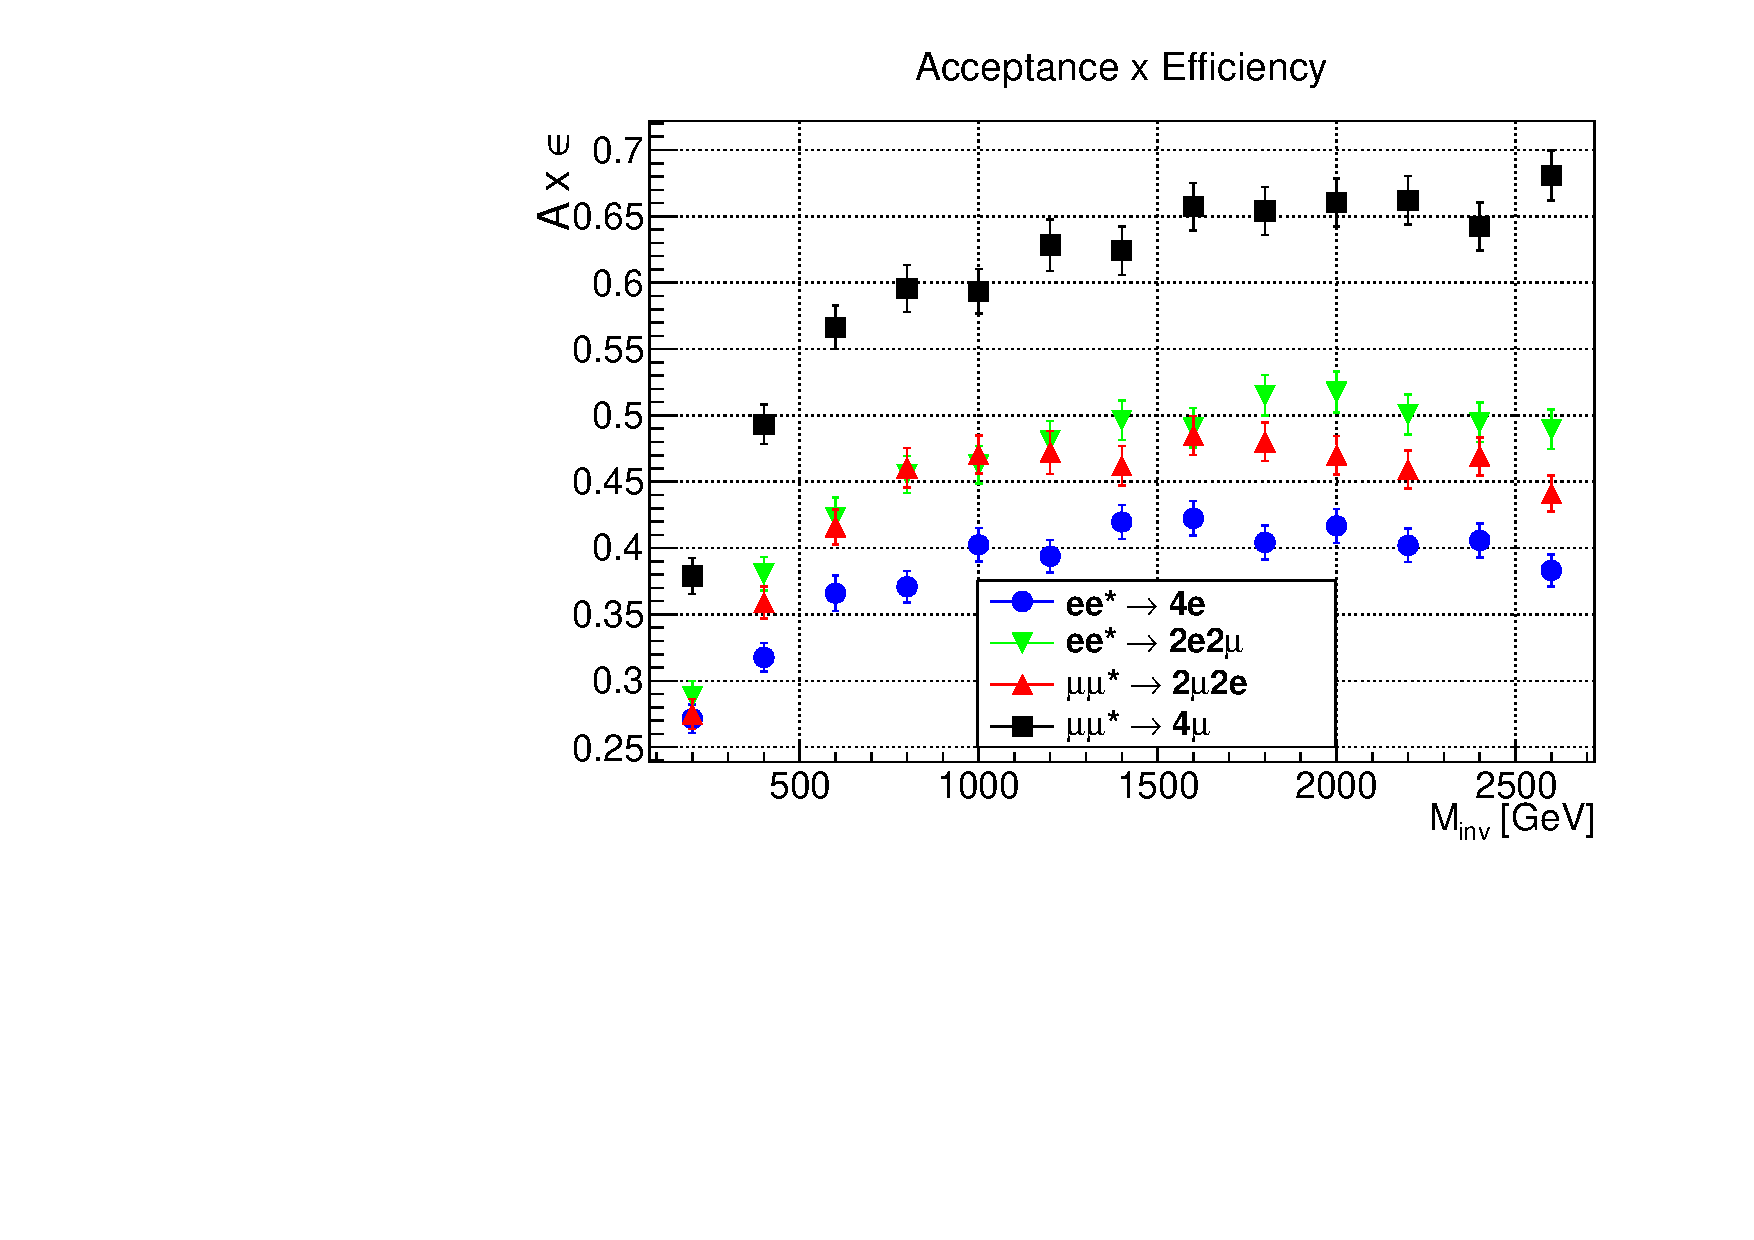
\includegraphics[width=0.9\textwidth]{plot/Effizienz_allchannels.pdf}
\end{center}
\caption{\label{fig:AccxEff}Total signal acceptance times efficiency ($A x \epsilon$) for the all selection criteria before final selection for the various signal samples.}
\end{figure}

\begin{figure}[h!]
\begin{center}
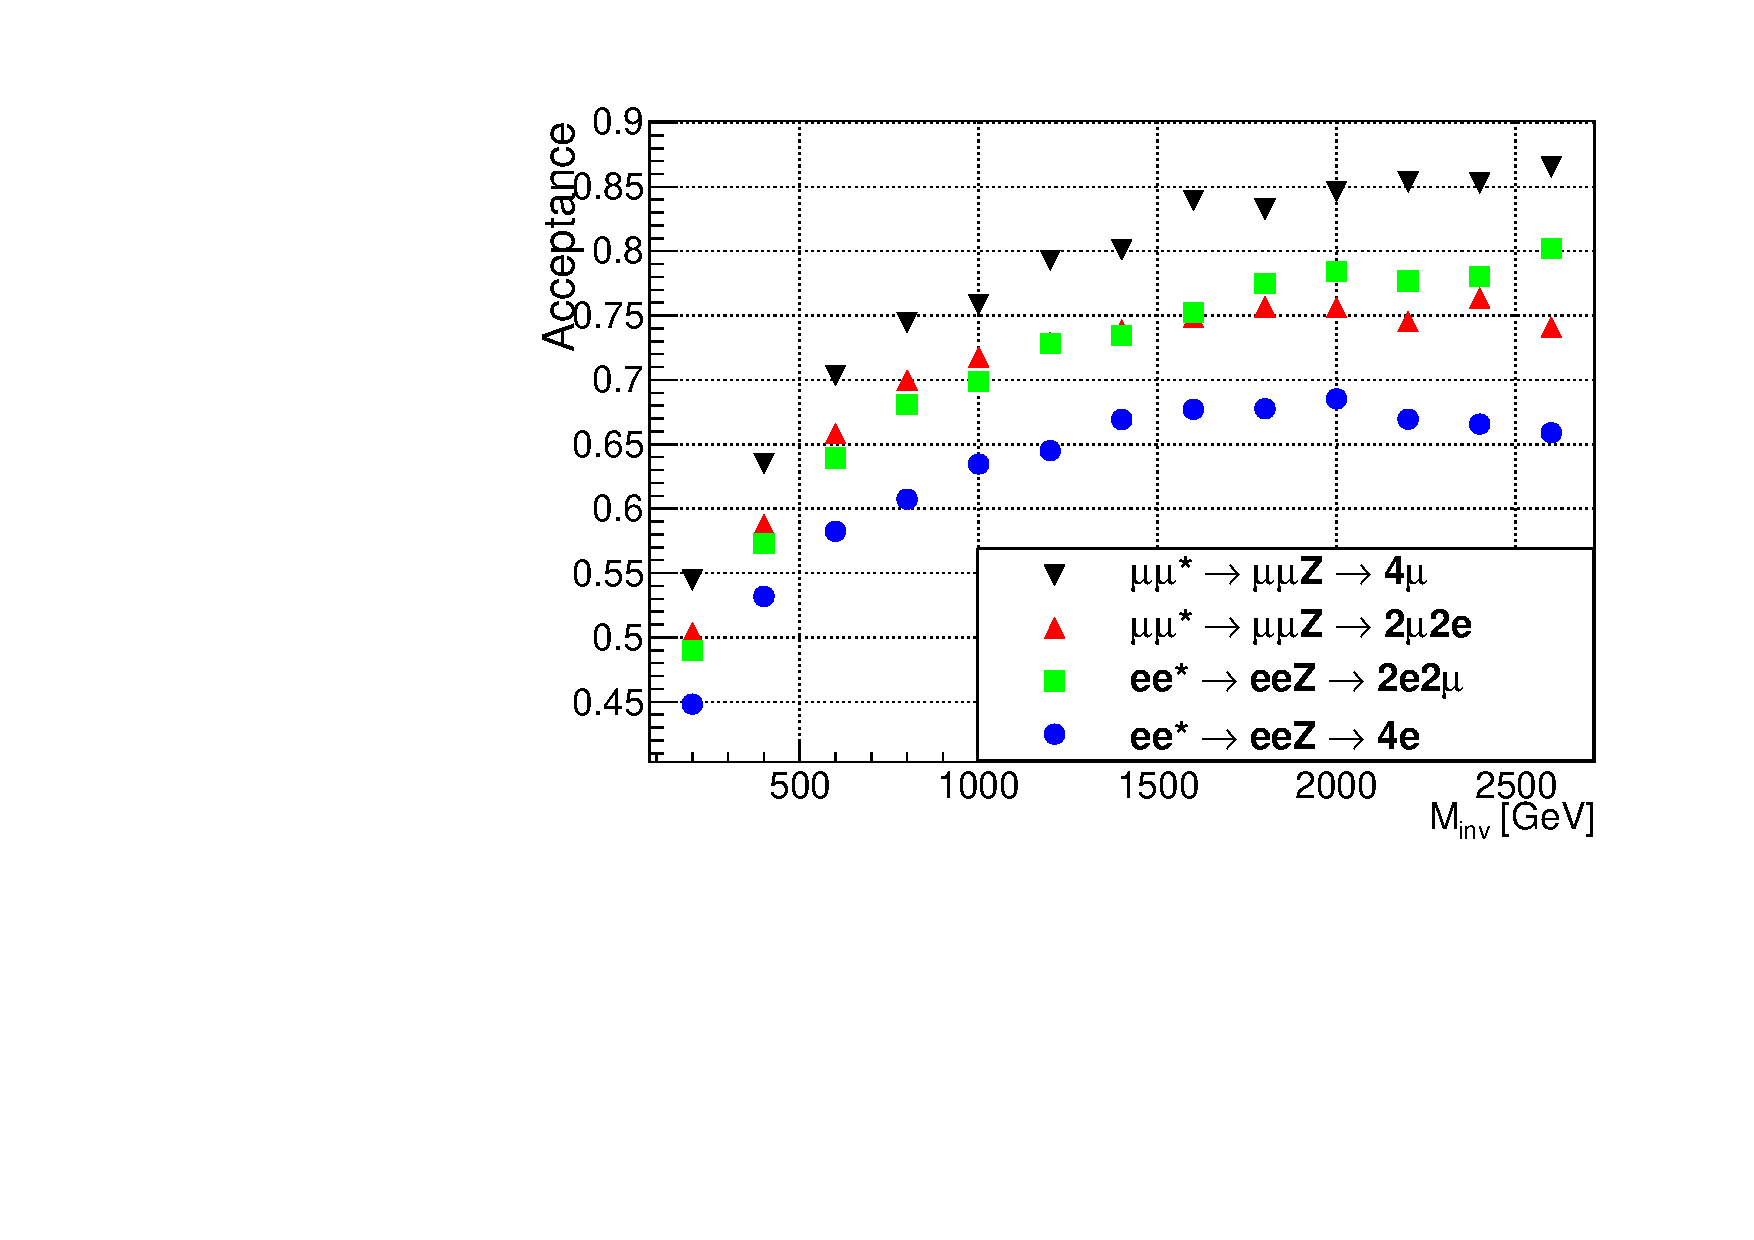
\includegraphics[width=0.9\textwidth]{plot/Acceptance_only.pdf}
\end{center}
\caption{\label{fig:Acc}Geometrical acceptance for all channels as given in the legend, with 4 muons and 2e2mu in the final state.}
\end{figure}

\clearpage

%%%%%%%%%%%%%%%%%%%%%%%%%%%%%%%%%%%%%%%%%%%%%%%%%%%%
\subsection{Background estimation}
\subsection*{After ID and isolation cuts}
%%%%%%%%%%%%%%%%%%%%%%%%%%%%%%%%%%%%%%%%%%%%%%%%%%%%

For a first comparison between data and background, the plots after applying the ID and isolation criteria for muons and electrons is shown. The plots in this section 
include scale factors for trigger, ID and isolation efficiencies and pileup re-weighting. Fig. \ref{fig:leptonPt} shows the distribution of the transverse momentum of the 
leptons. Fig. \ref{fig:leptonEta} shows the $\eta$ distribution of the leptons while \ref{fig:leptonPhi} shows the $\phi$ distribution. The distribution for the 
reconstructed Z is given in Fig. \ref{fig:MinvZ}. Fig. \ref{fig:MinvnoZ} shows the invariant mass distribution of the non-Z lepton pair where the Z veto will be placed. As one can see from this plot, most signal events lays on the high invariant mass region beyond 106 GeV. 
Additionally, Fig. \ref{fig:Minv4mu} and Fig. \ref{fig:ZdR} show the invariant mass of all four leptons and the $\Delta R$ of the two muons from the Z decay. In all 
distributions, data and background are in same shape and agree with each other. 

In Tab. \ref{tab:yieldsmustar} and Tab. \ref{tab:yieldsestar} the contribution of each background can be seen for the two $\mu^{*}$ and the two $e^{*}$ channels, and several sets of expected yield of signal at $\Lambda = M_{\ell^{*}}$ are provided as well. In the 4e channel, the agreement between data and MC is good. The $4\mu$ channel has a small 
downward-fluctuation in data and the mixed channels have an upward-fluctuation in data. The fluctuation in the mixed channels has been investigated by changing the $p_{T}$  
cuts, using other ID (for example MVA electron ID) and doing comparisons to other analyses. The excess comes mainly from the region about 200 GeV in the four lepton invariant mass 
distribution. In this region, other analyses such as $H\rightarrow ZZ\rightarrow 4l$ (see Fig. \ref{fig:HIGref})\cite{HIGxcess} do also observe an upward-fluctuation.          

\begin{table}[h!]
\begin{center}
\begin{tabular}{|l|l|l|l|}
\hline 
Background & $\mu\mu^{*}\rightarrow 4\mu$ & $\mu\mu^{*}\rightarrow 2\mu 2e$ & combined \\ 
\hline
$ZZ \rightarrow 4\mu$ & $33.82\pm 0.18$ & $0.00\pm 0.00$ & $33.82\pm 0.18$ \\
$ZZ \rightarrow 2e 2\mu$ & $0.00\pm 0.00$ & $50.07\pm 0.34$ & $50.07\pm 0.34$ \\
$ZZ \rightarrow 2e 2\tau$ & $0.00\pm 0.00$ & $0.09\pm 0.02$ & $0.09\pm 0.02$\\
$ZZ \rightarrow 2\mu 2\tau$ & $0.13\pm 0.02$ & $0.17\pm 0.03$ & $0.30\pm 0.04$\\
$WZ \rightarrow 3l \nu$ & $0.00\pm 0.00$ & $0.47\pm 0.07$ & $0.47\pm 0.07$\\
$gg \rightarrow ZZ \rightarrow 2l2l'$ & $0.01\pm 0.00$ & $3.64\pm 0.05$ & $3.65\pm 0.05$\\
$gg \rightarrow ZZ \rightarrow 4l$ & $1.84\pm 0.02$ & $0.01\pm 0.00$ & $1.85\pm 0.02$\\
$ttZ$ & $0.45\pm 0.10$ & $0.63\pm 0.10$ & $1.07\pm 0.14$\\
$ttWW$ & $0.00\pm 0.00$ & $0.01\pm 0.00$ & $0.01\pm 0.00$\\
$WWZ$ & $0.16\pm 0.03$ & $0.26\pm 0.04$ & $0.42\pm 0.05$\\
$WZZ$ & $0.10\pm 0.01$ & $0.17\pm 0.02$ & $0.27\pm 0.02$\\
$ZZZ$ & $0.07\pm 0.01$ & $0.12\pm 0.01$ & $0.19\pm 0.01$\\
$DYJet$ & $0.00\pm 0.00$ & $0.55\pm 0.55$ & $0.55\pm 0.55$\\
\hline
Total & $36.63\pm 0.23$ & $56.19\pm 0.37$ & $92.82\pm 0.42$\\
Total (with systematics) & $36.63\pm 4.86$ & $56.19\pm 7.01$ & $92.82\pm 8.53$\\
\hline
\hline
Data & 29 & 66 & 95\\
\hline
\hline
$M_{\mu^{*}}$ = 200 GeV & $2.9 \times 10^{5}$  & $2.1 \times 10^{5}$ & $5.0 \times 10^{5}$\\
$M_{\mu^{*}}$ = 1000 GeV & $1.2 \times 10^{2}$ & $9.3 \times 10^{1}$ & $2.1 \times 10^{2}$\\
$M_{\mu^{*}}$ = 1800 GeV & 1.36 & 1.08 & 2.44\\
$M_{\mu^{*}}$ = 2600 GeV & 0.04 & 0.03 & 0.07\\
\hline
\end{tabular}
\end{center}
\caption{\label{tab:yieldsmustar}Event yields for $\mu\mu^{*}\rightarrow 4\mu$ and $\mu\mu^{*}\rightarrow 2\mu 2e$ without invariant mass cut. If the column includes $0.00 \pm 0.00$ events, the calculated number is to small for a prediction.}
\end{table}


\begin{table}[h!]
\begin{center}
\begin{tabular}{|l|l|l|l|}
\hline 
Background & $e e^{*}\rightarrow 4e$ & $e e^{*}\rightarrow 2e 2\mu$ & combined \\ 
\hline
$ZZ \rightarrow 4e$ & $18.65\pm 0.13$ & $0.00\pm 0.00$ & $18.65\pm 0.13$\\
$ZZ \rightarrow 2e 2\mu$ & $0.00\pm 0.00$ & $50.97\pm 0.35$ & $50.97\pm 0.35$\\
$ZZ \rightarrow 2e 2\tau$ & $0.10\pm 0.02$ & $0.10\pm 0.02$ & $0.20\pm 0.04$\\
$ZZ \rightarrow 2\mu 2\tau$ & $0.00\pm 0.00$ & $0.18\pm 0.03$ & $0.18\pm 0.03$\\
$WZ \rightarrow 3l \nu$ & $0.03\pm 0.02$ & $0.47\pm 0.07$ & $0.50\pm 0.07$ \\
$gg \rightarrow ZZ \rightarrow 2l2l'$ & $0.01\pm 0.01$ & $3.68\pm 0.05$ & $3.69\pm 0.05$ \\
$gg \rightarrow ZZ \rightarrow 4l$ & $1.12\pm 0.01$ & $0.01\pm 0.00$ & $1.13\pm 0.01$\\
$ttZ$ & $0.21\pm 0.06$ & $0.76\pm 0.13$ & $0.97\pm 0.14$\\
$ttWW$ & $0.00\pm 0.00$ & $0.01\pm 0.00$ & $0.01\pm 0.00$\\
$WWZ$ & $0.00\pm 0.00$ & $0.25\pm 0.04$ & $0.25\pm 0.04$\\
$WZZ$ & $0.02\pm 0.01$ & $0.17\pm 0.02$ & $0.19\pm 0.02$\\
$ZZZ$ & $0.03\pm 0.00$ & $0.12\pm 0.01$ & $0.15\pm 0.01$\\
$DYJet$ & $0.00\pm 0.00$ & $0.55\pm 0.55$ & $0.55\pm 0.55$\\
\hline
Total & $20.17\pm 0.15$ & $57.27\pm 0.37$ & $78.44\pm 0.40$\\
Total (with systematics) & $20.17\pm 2.84$ & $57.27\pm 7.81$ & $78.44\pm 8.31$ \\
\hline
\hline
Data & 16 & 67 & 83\\
\hline
\hline
$M_{e^{*}}$ = 200 GeV & $2.1 \times 10^{5}$  & $2.2 \times 10^{5}$ & $4.3 \times 10^{5}$\\
$M_{e^{*}}$ = 1000 GeV & $7.8 \times 10^{1}$ & $8.7 \times 10^{1}$ & $1.7 \times 10^{2}$\\
$M_{e^{*}}$ = 1800 GeV & 0.86 & 1.08 & 1.94\\
$M_{e^{*}}$ = 2600 GeV & 0.03 & 0.03 & 0.06\\
\hline
\end{tabular}
\end{center}
\caption{\label{tab:yieldsestar}Events yields for $e e^{*}\rightarrow 4e$ and $e e^{*}\rightarrow 2e 2\mu$ without invariant mass cut. If the column includes $0.00 \pm 0.00$ events, the calculated number is to small for a prediction.}
\end{table}


\begin{figure}[hp!]
\begin{center}
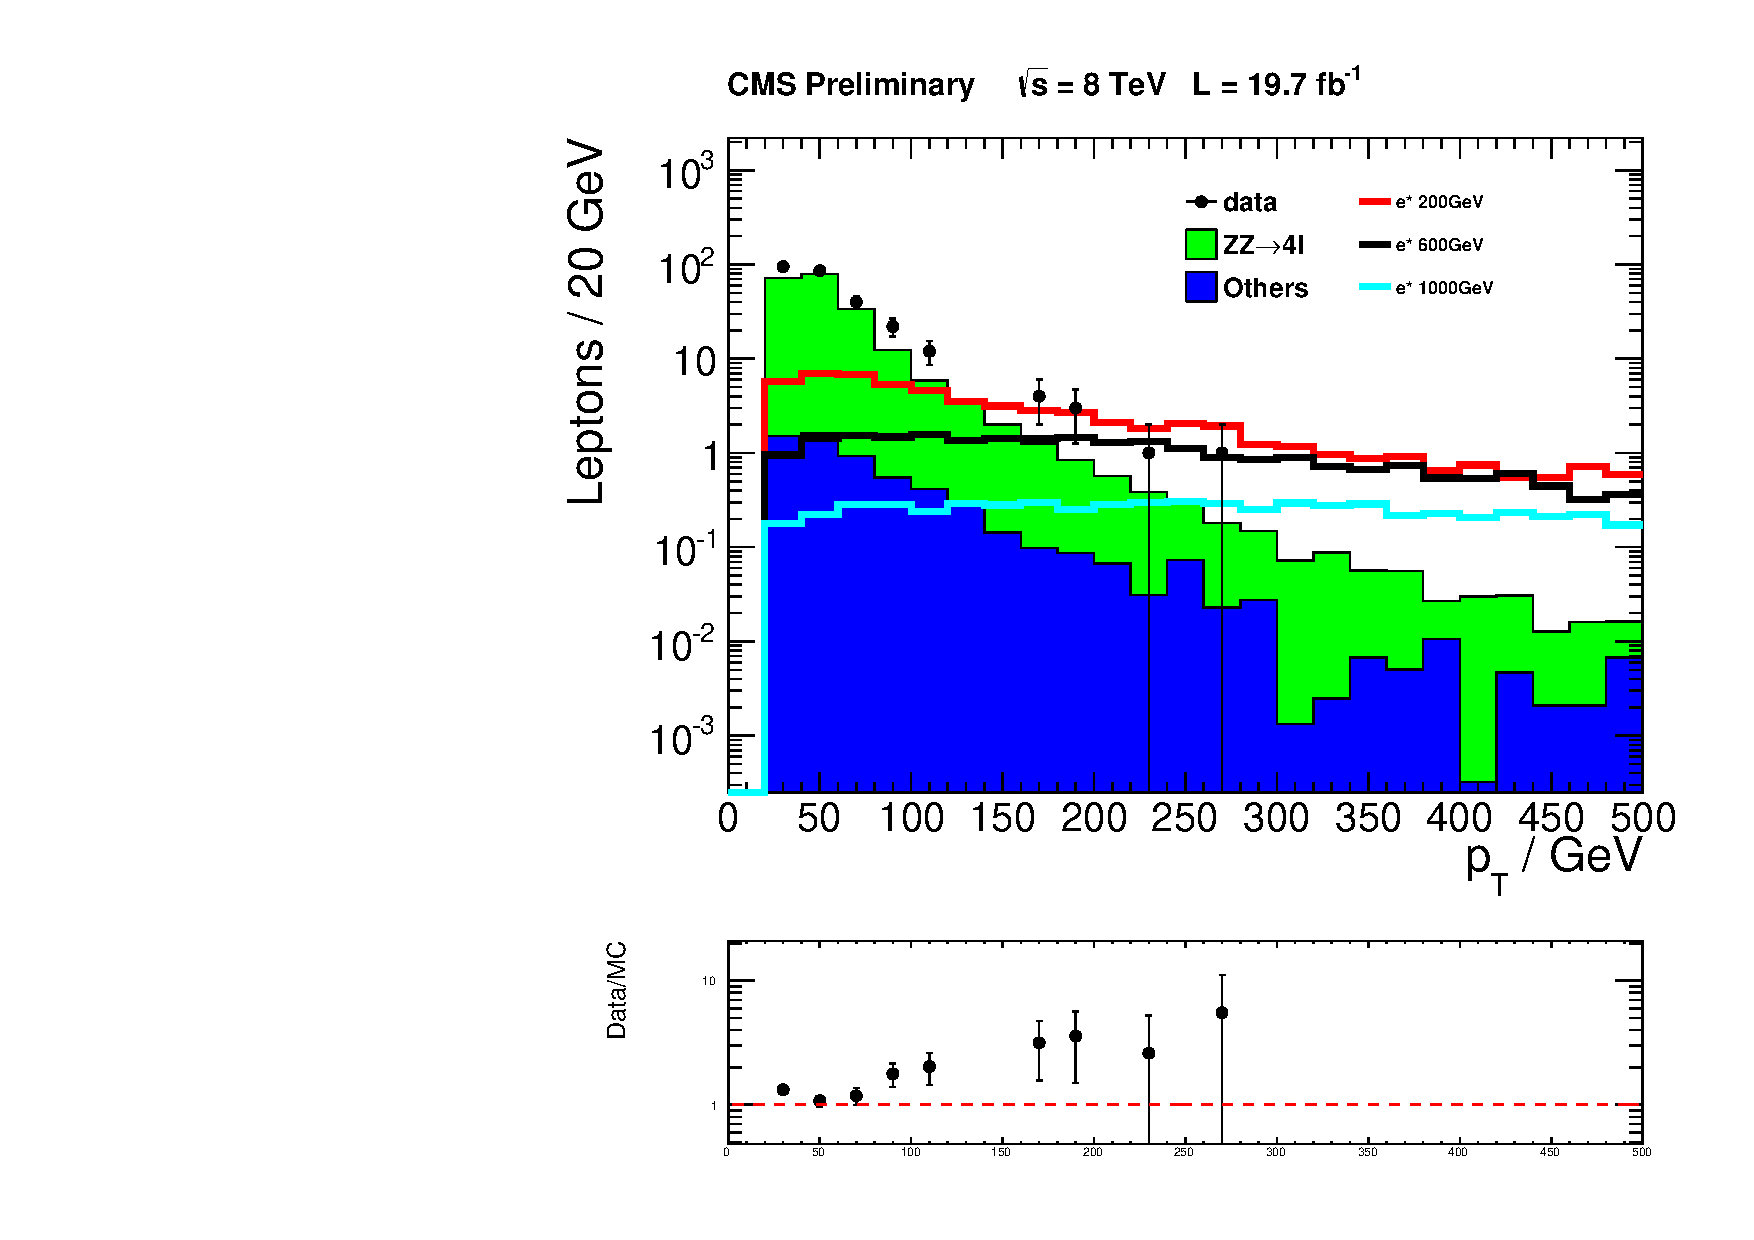
\includegraphics[width=0.48\textwidth]{plot/Pt_2mu2e.pdf} 
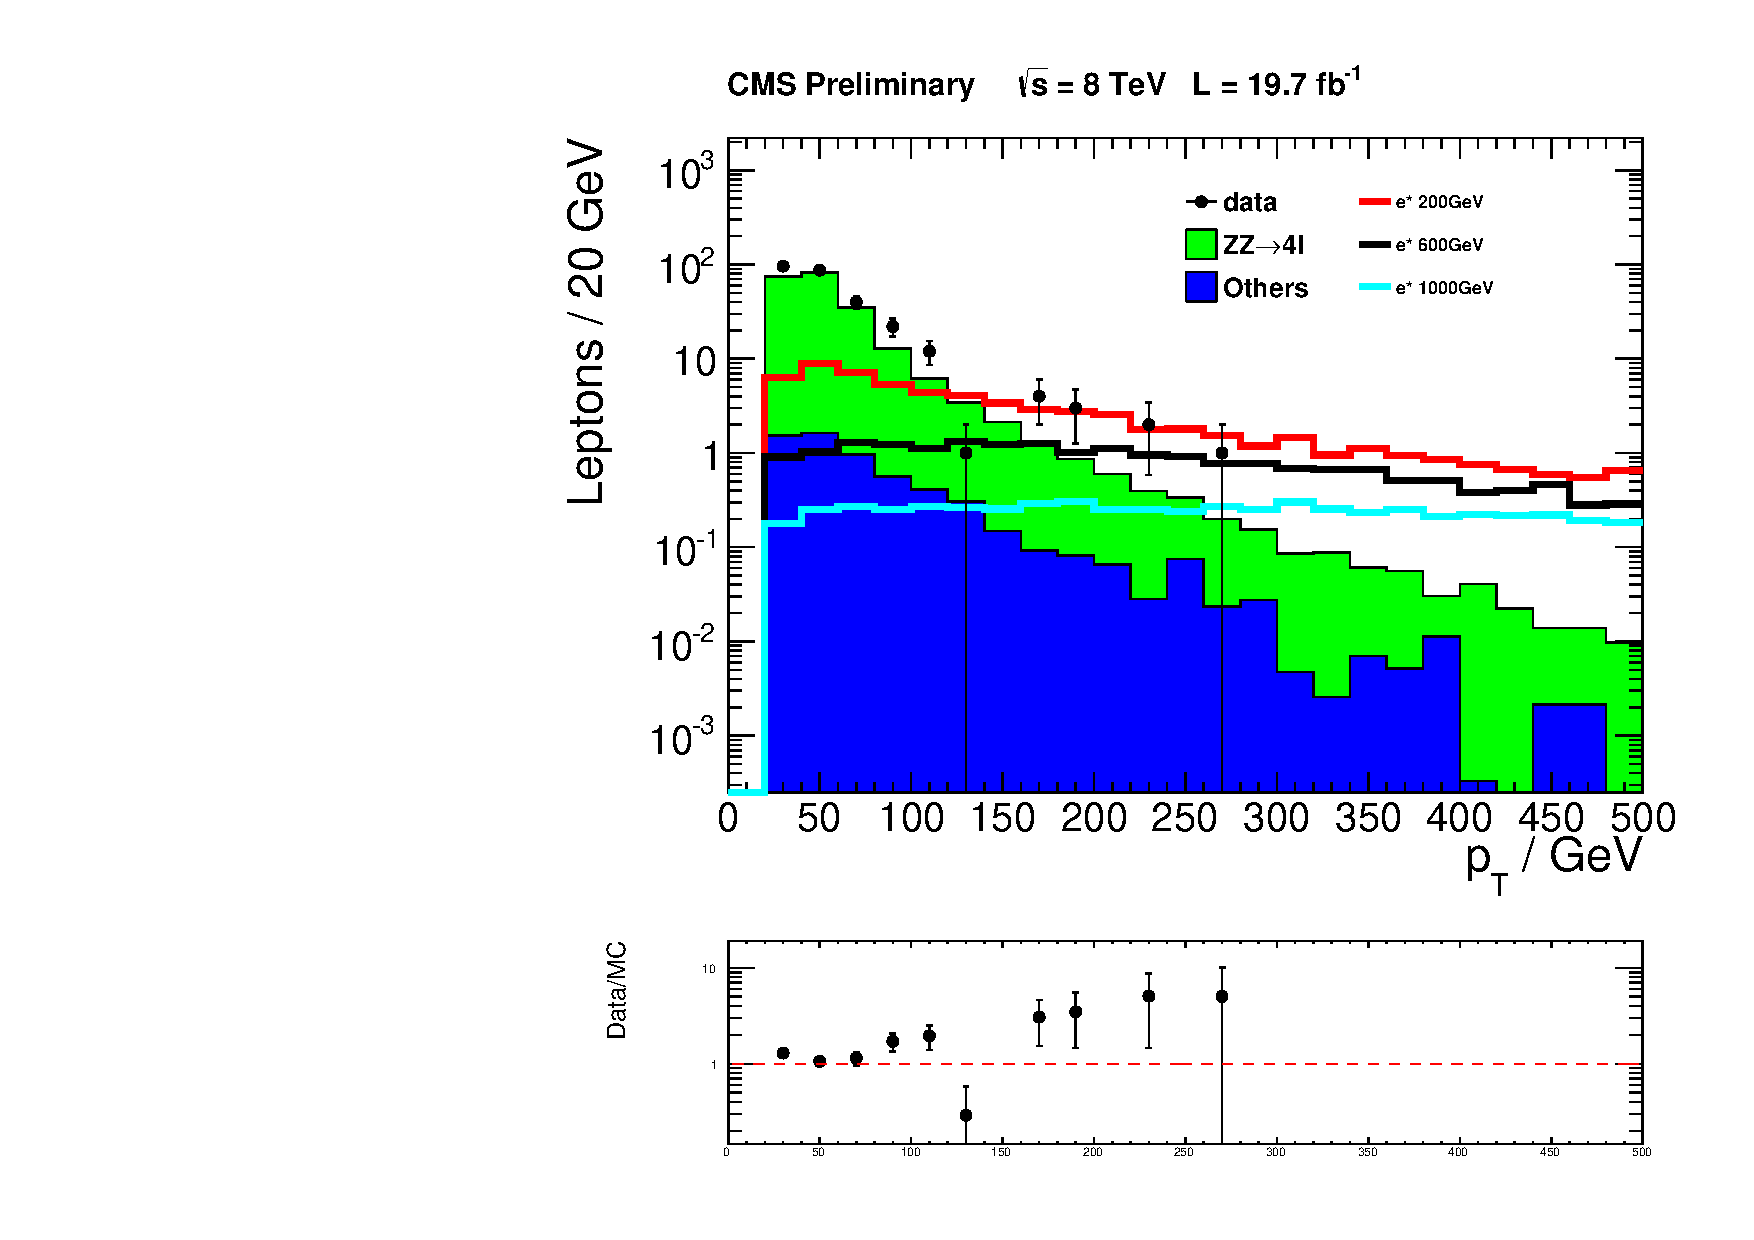
\includegraphics[width=0.48\textwidth]{plot/Pt_2e2mu.pdf}
\end{center}
\caption{\label{fig:leptonPt}Lepton $p_{T}$ before invariant mass cuts. Left: $\mu\mu^{*}\rightarrow 2\mu2e$ channel, Right: $ee^{*}\rightarrow 2e2\mu$ channel}
\end{figure}


\begin{figure}[hp!]
\begin{center}
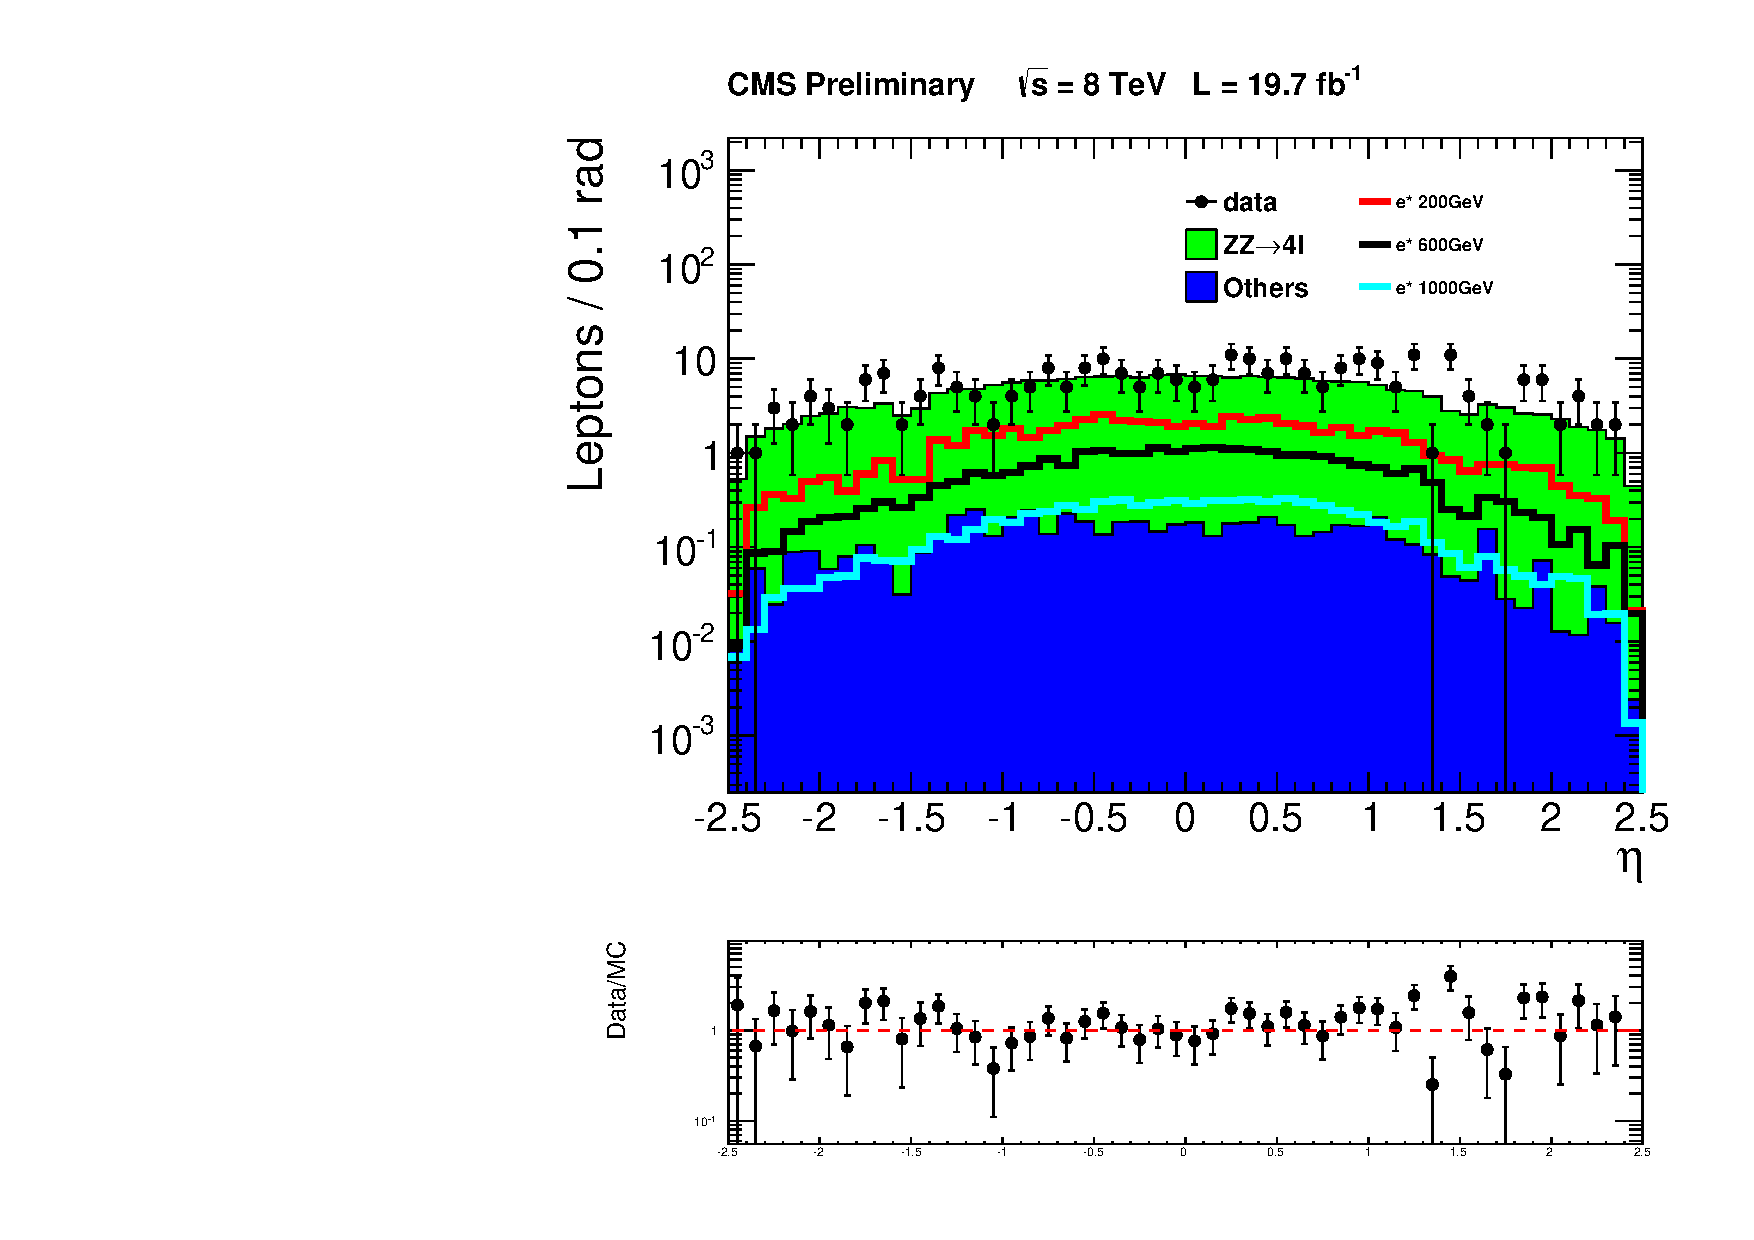
\includegraphics[width=0.48\textwidth]{plot/Eta_2mu2e.pdf} 
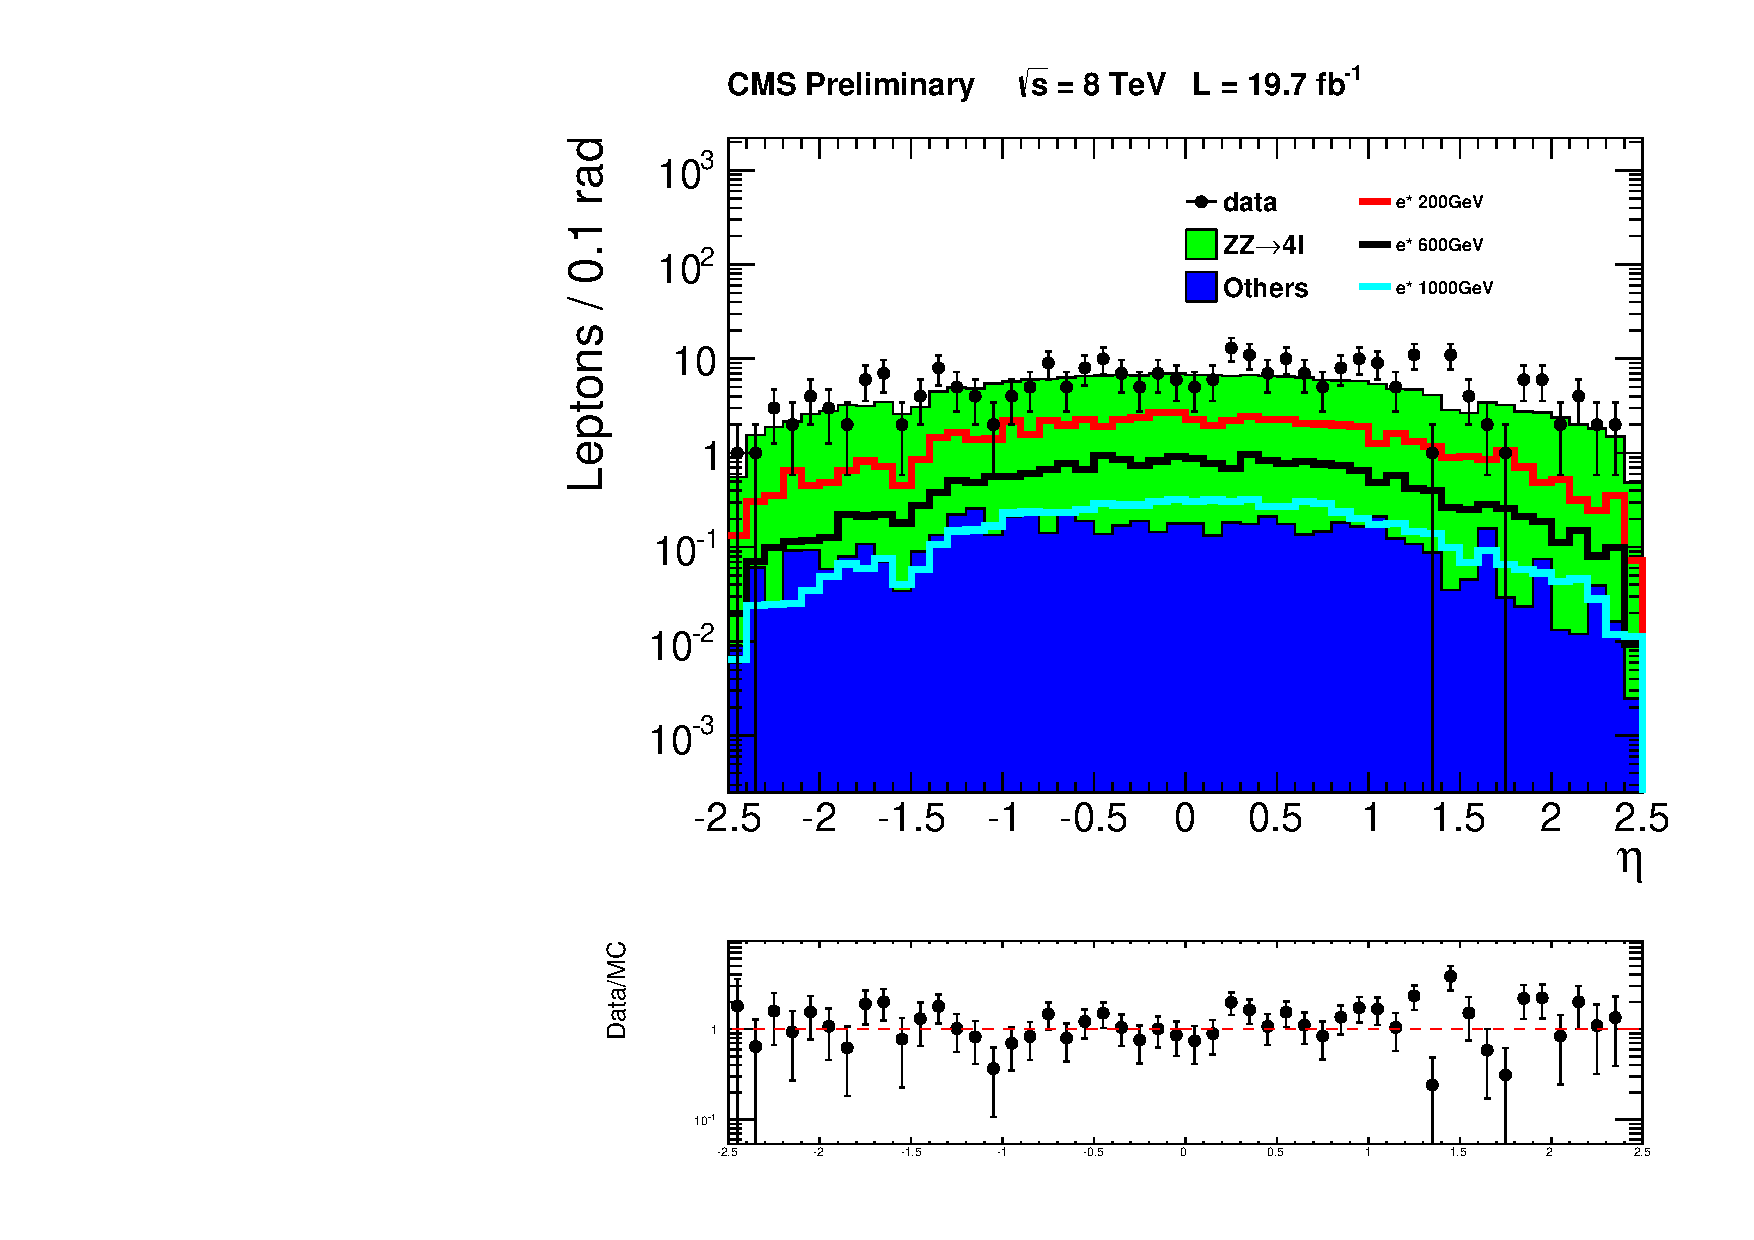
\includegraphics[width=0.48\textwidth]{plot/Eta_2e2mu.pdf}
\end{center}
\caption{\label{fig:leptonEta}Lepton $\eta$ before invariant mass cuts. Left: $\mu\mu^{*}\rightarrow 2\mu2e$ channel, Right: $ee^{*}\rightarrow 2e2\mu$ channel}
\end{figure}


\begin{figure}[hp!]
\begin{center}
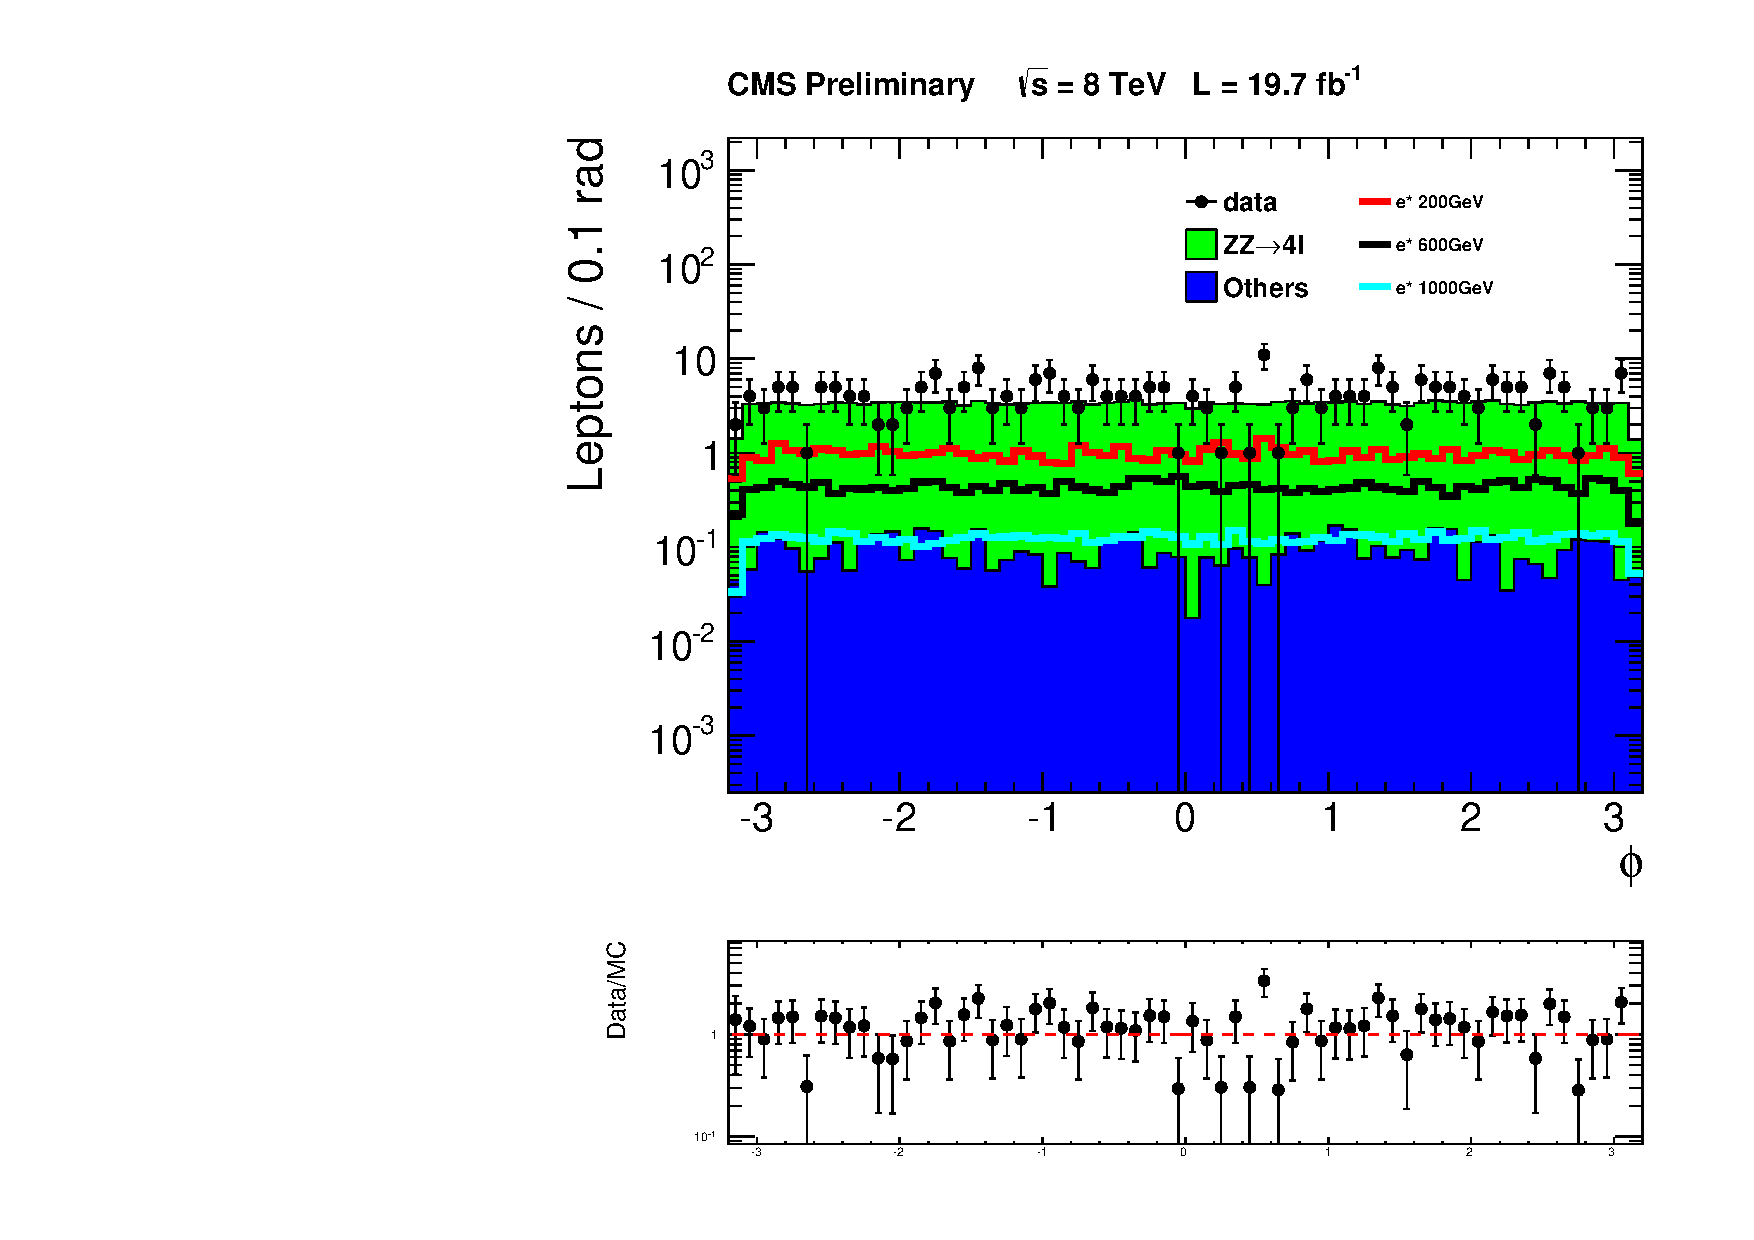
\includegraphics[width=0.48\textwidth]{plot/Phi_2mu2e.pdf} 
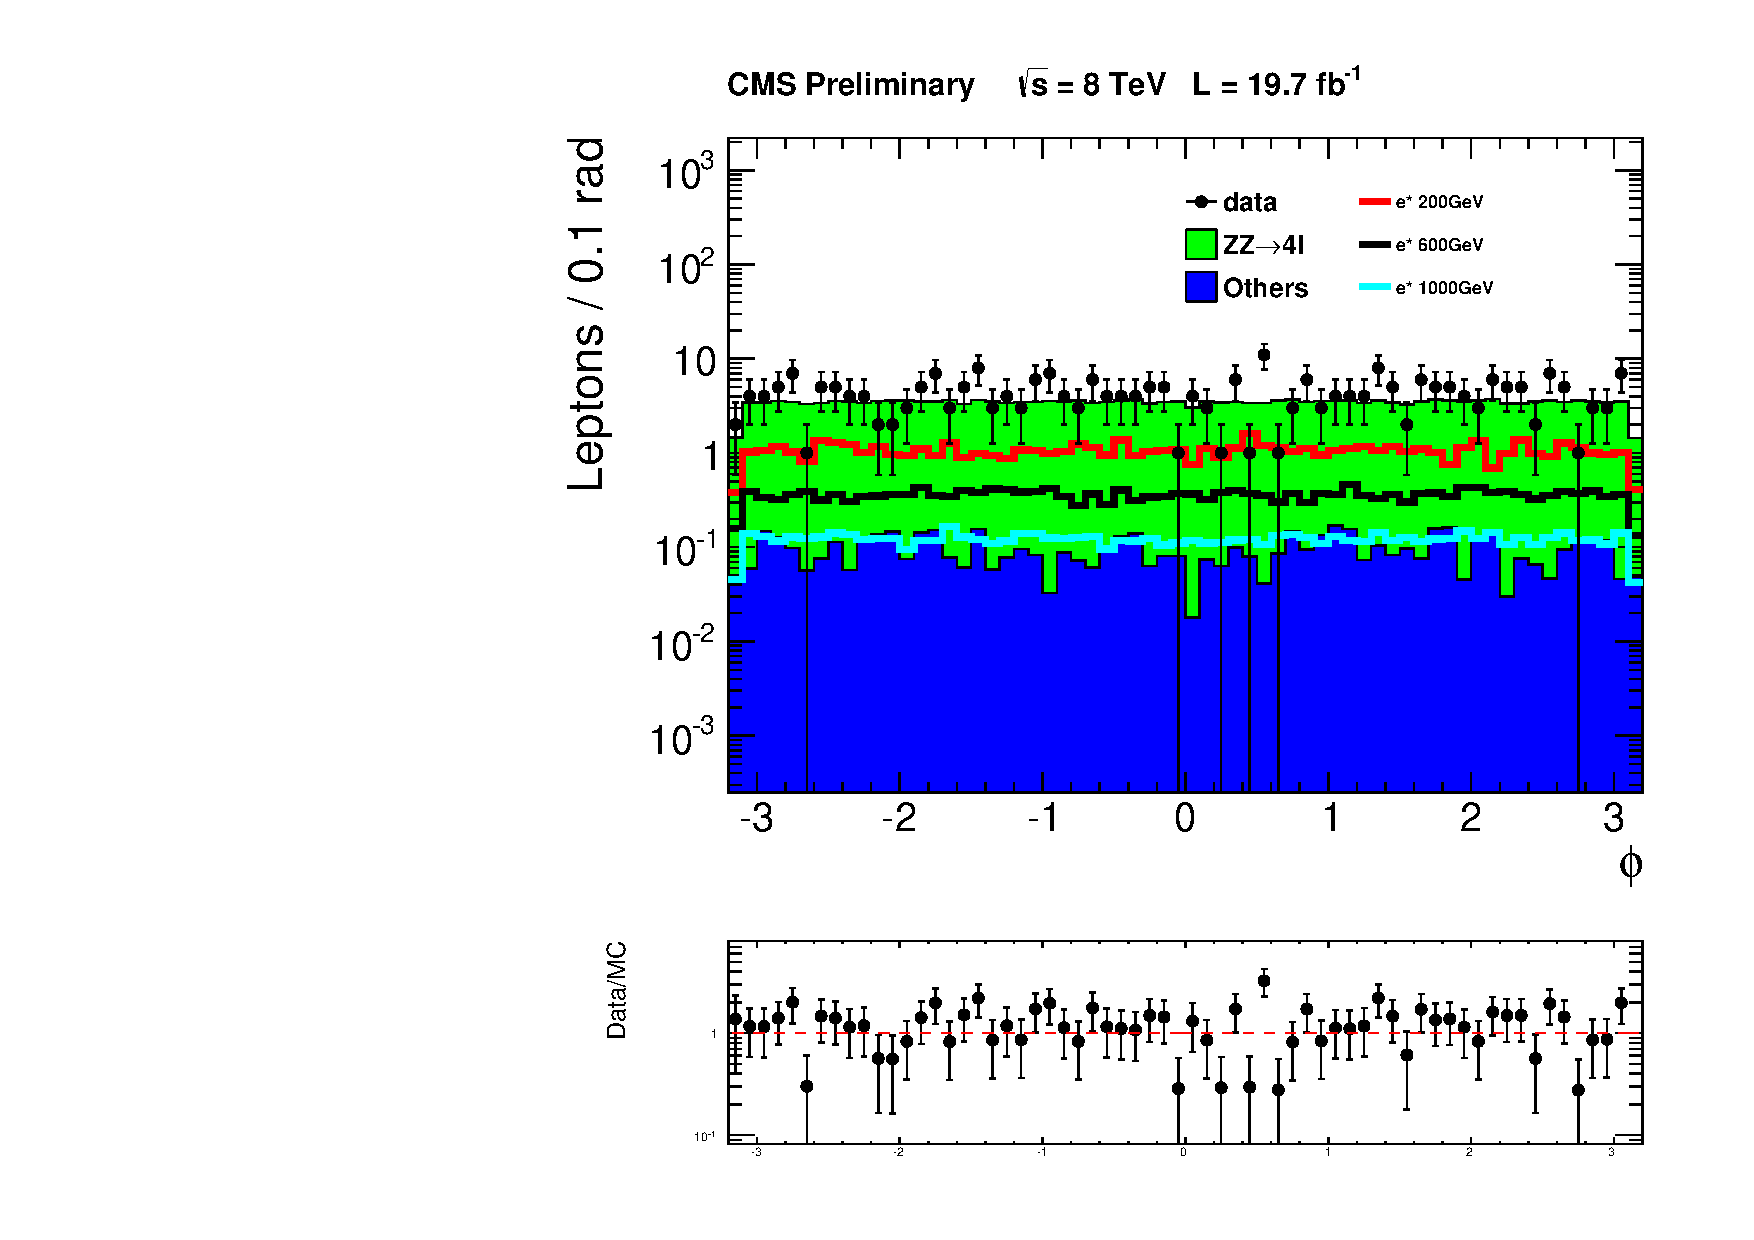
\includegraphics[width=0.48\textwidth]{plot/Phi_2e2mu.pdf}
\end{center}
\caption{\label{fig:leptonPhi}Lepton $\phi$ before invariant mass cuts. Left: $\mu\mu^{*}\rightarrow 2\mu2e$ channel, Right: $ee^{*}\rightarrow 2e2\mu$ channel}
\end{figure}


\begin{figure}[hp!]
\begin{center}
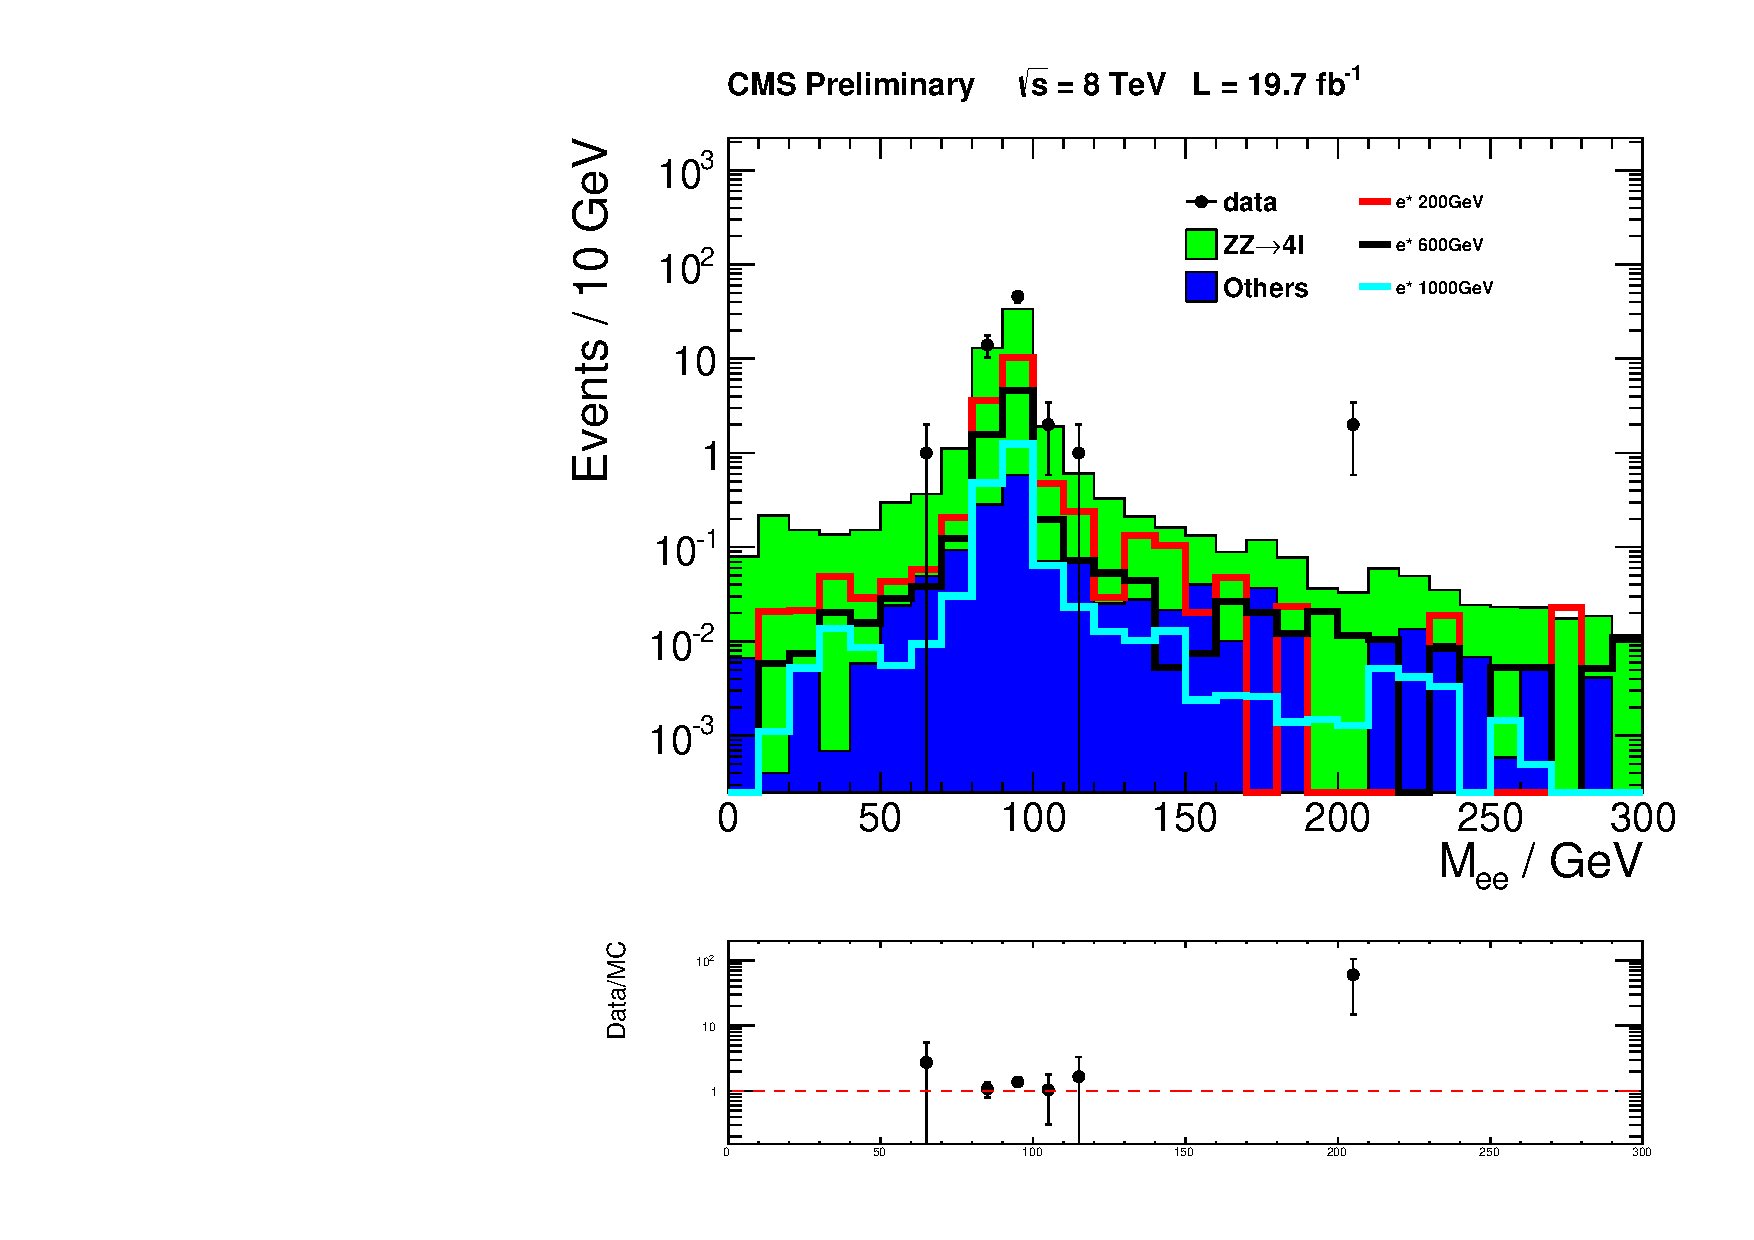
\includegraphics[width=0.48\textwidth]{plot/Z_2mu2e.pdf} 
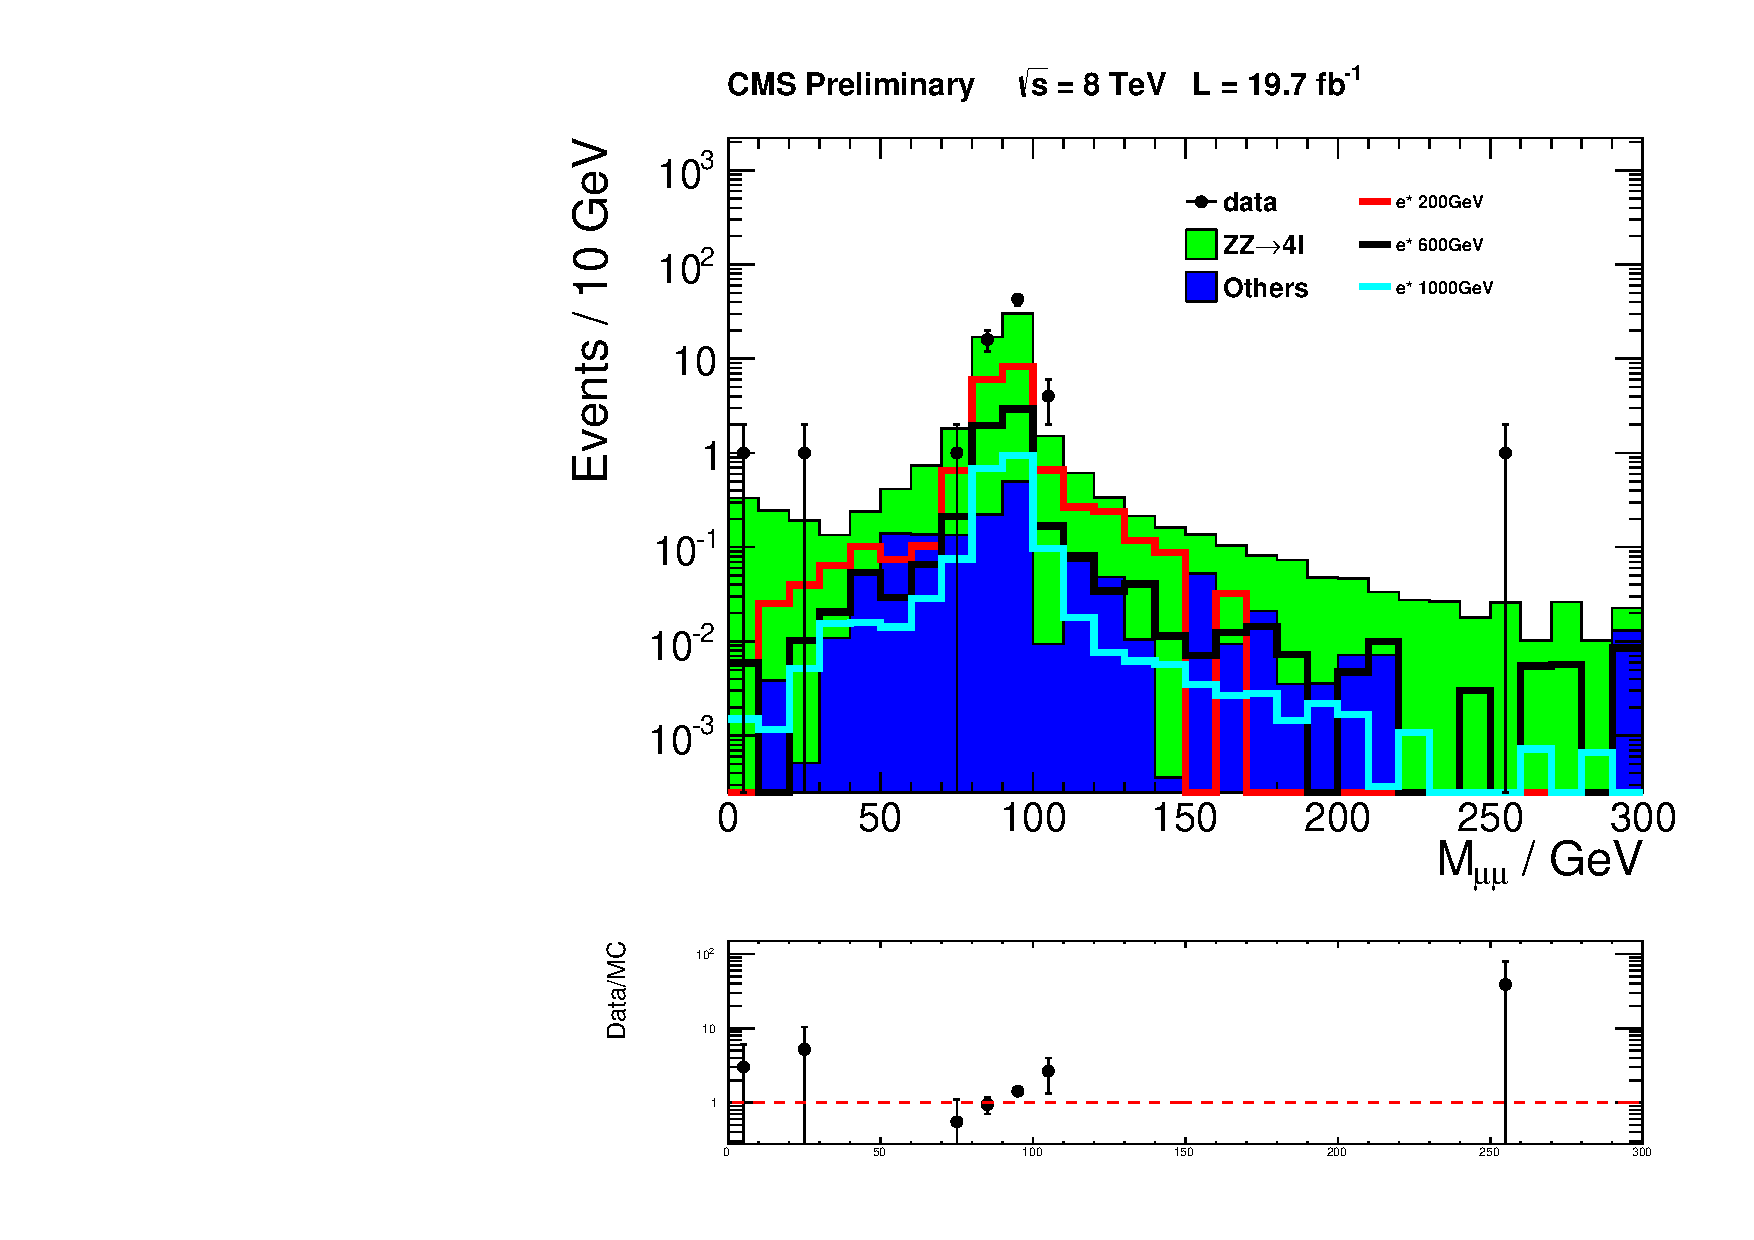
\includegraphics[width=0.48\textwidth]{plot/Z_2e2mu.pdf}
\end{center}
\caption{\label{fig:MinvZ}Invariant mass distribution of the selected Z before invariant mass cuts. Left: $\mu\mu^{*}\rightarrow 2\mu2e$ channel, Right: $ee^{*}\rightarrow 2e2\mu$ channel}
\end{figure}


\begin{figure}[hp!]
\begin{center}
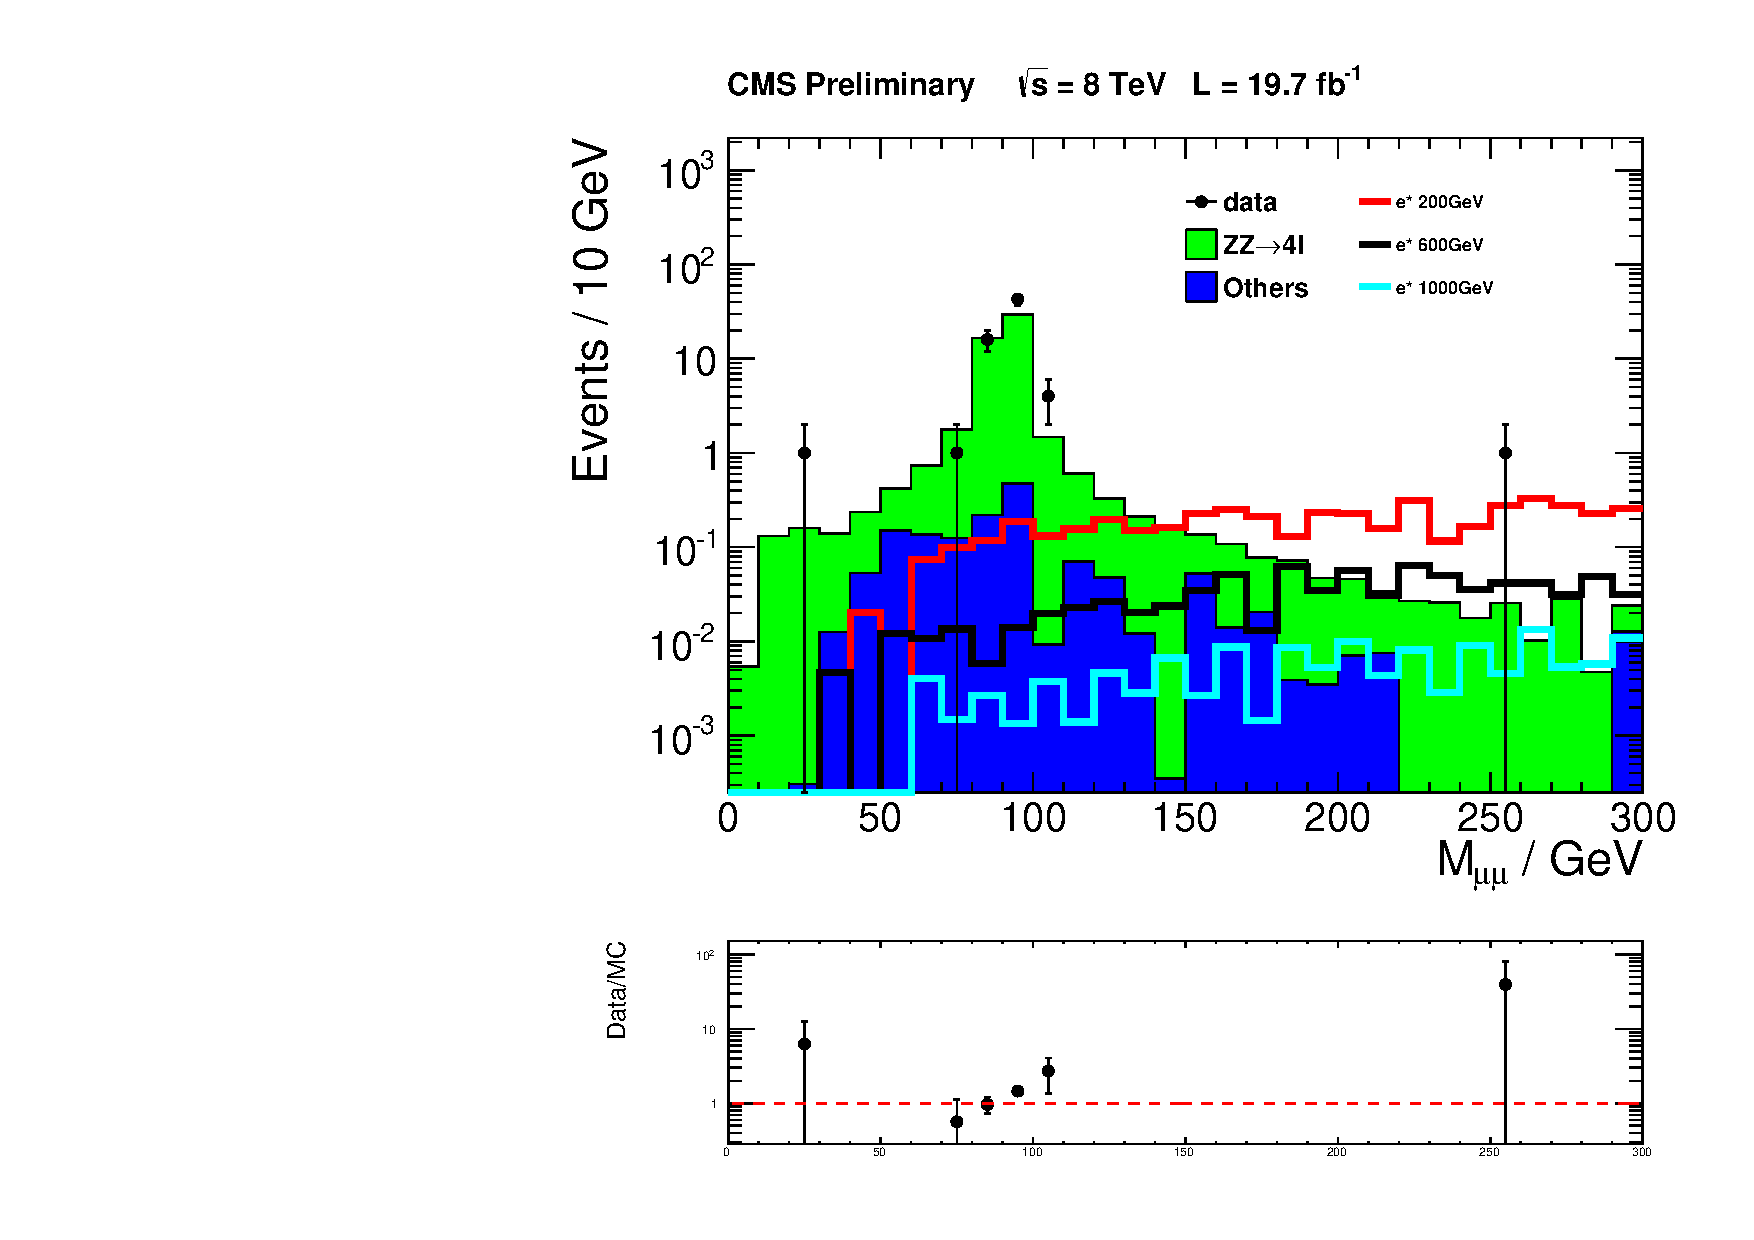
\includegraphics[width=0.48\textwidth]{plot/nonZ_2mu2e.pdf} 
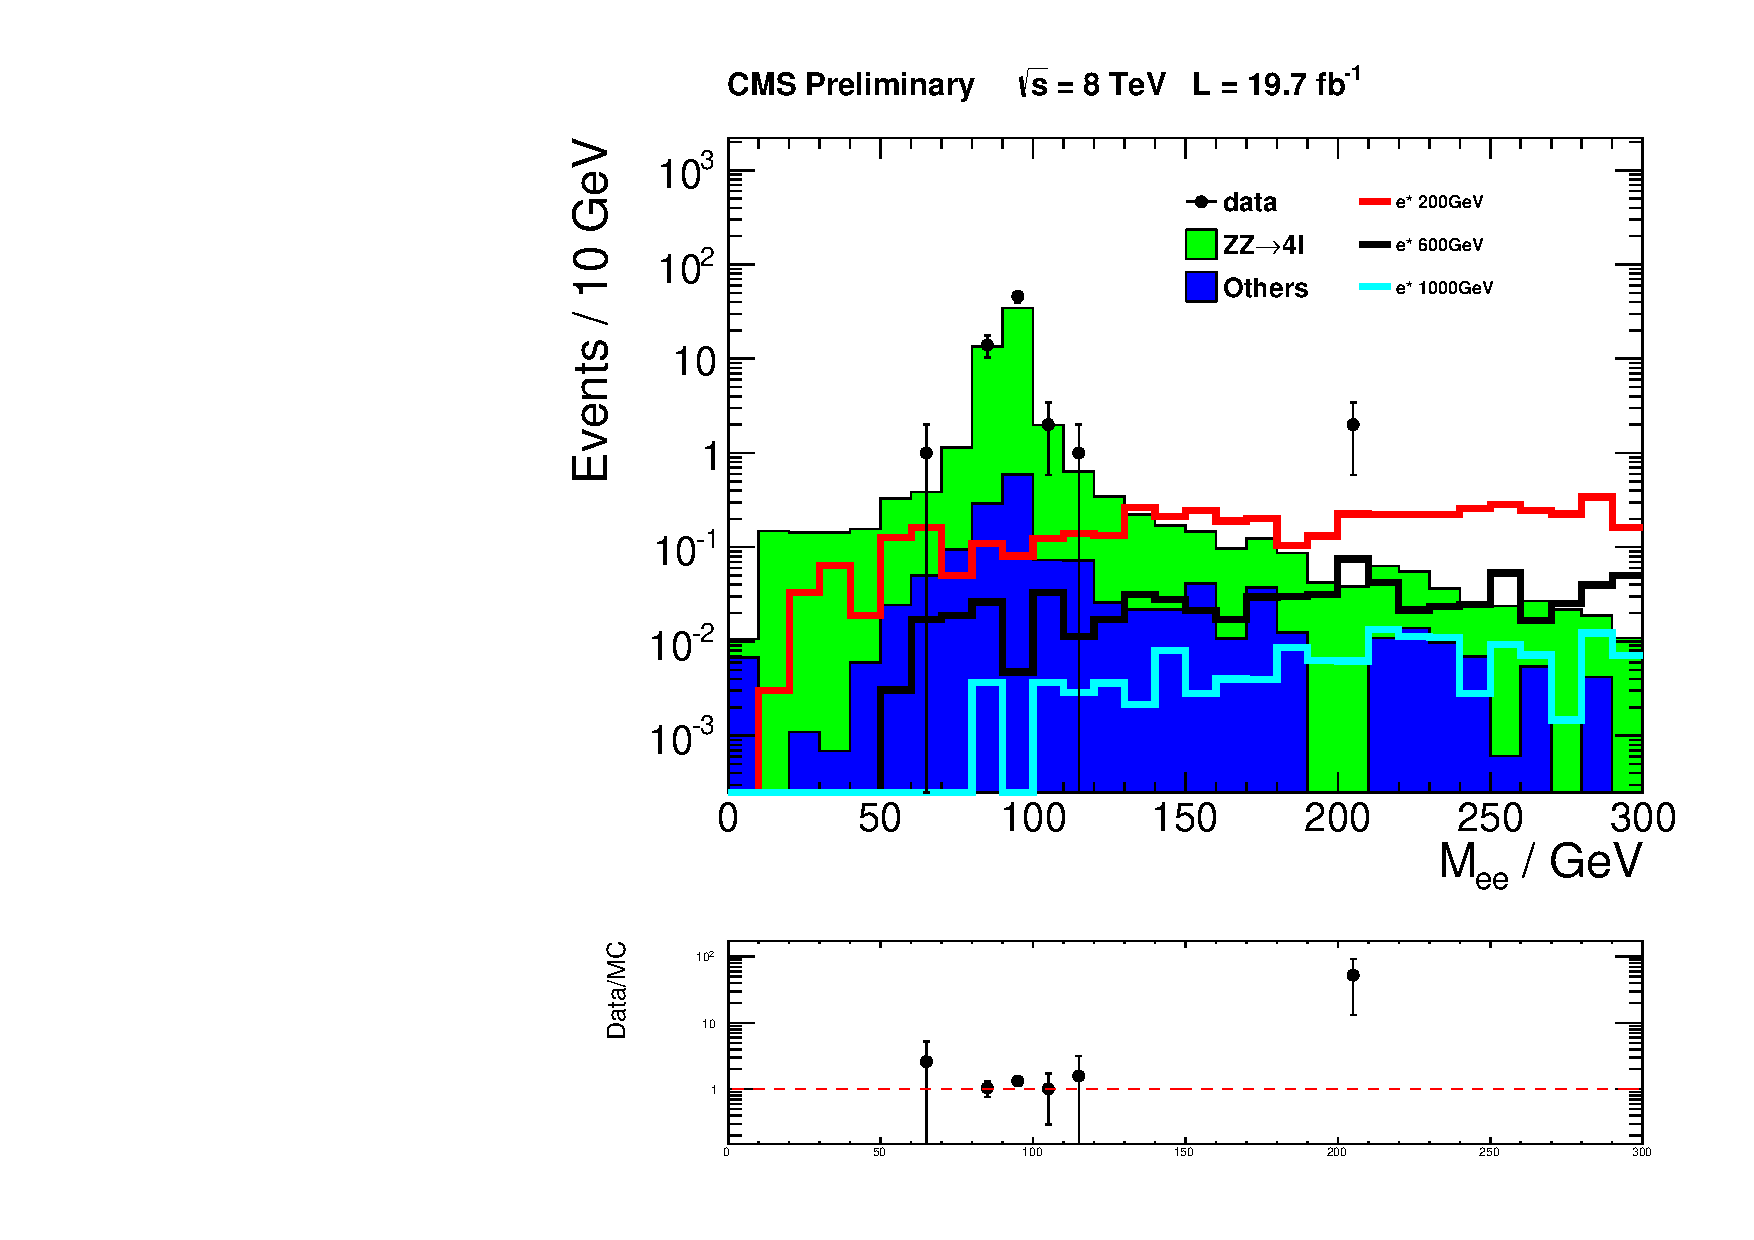
\includegraphics[width=0.48\textwidth]{plot/nonZ_2e2mu.pdf}
\end{center}
\caption{\label{fig:MinvnoZ}Invariant mass distribution of the vetoed Z before invariant mass cuts. Left: $\mu\mu^{*}\rightarrow 2\mu2e$ channel, Right: $ee^{*}\rightarrow 2e2\mu$ channel}
\end{figure}

%\begin{figure}[hp!]
%\begin{center}
%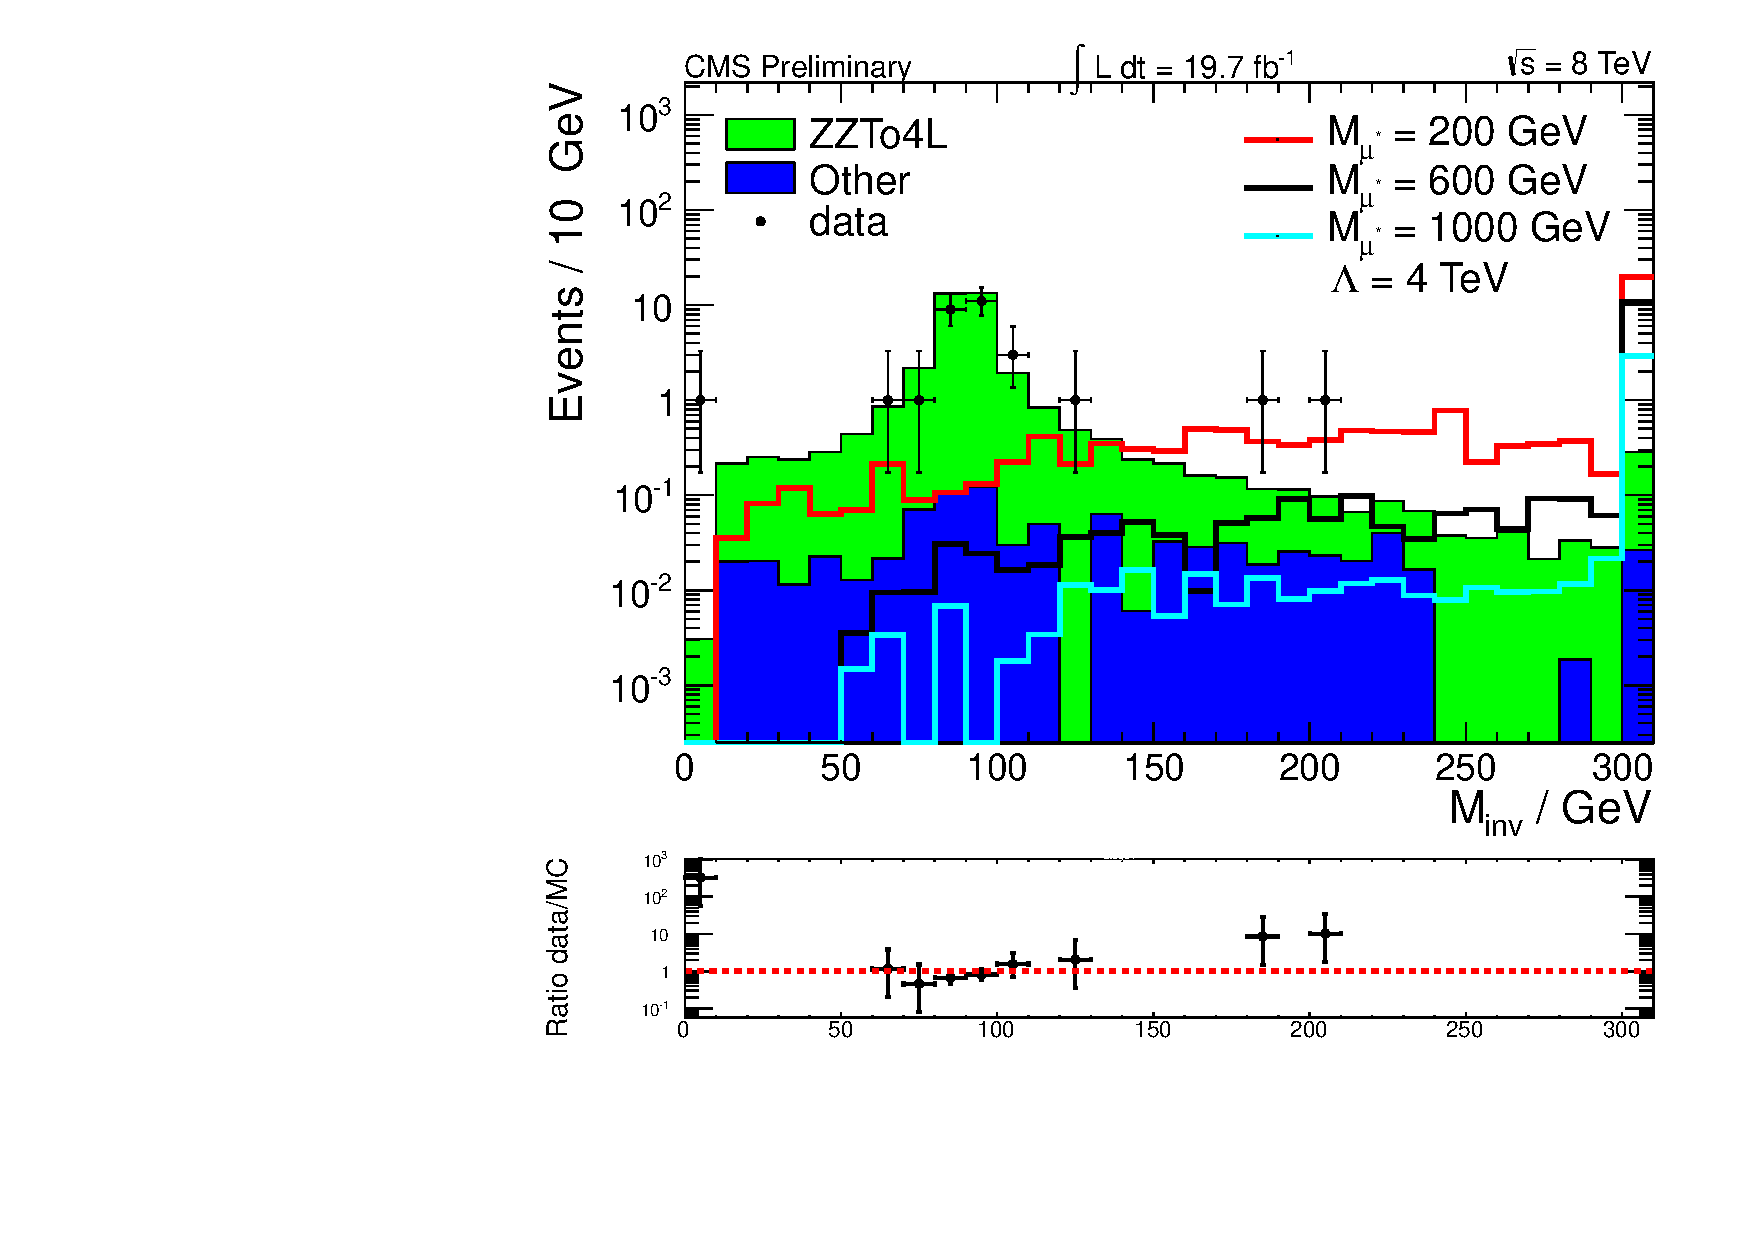
\includegraphics[width=0.65\textwidth]{plots/nonZLog_4mu.pdf}
%\end{center}
%\caption{\label{fig:MinvnoZLog_4mu}Invariant mass distribution of the vetoed Z for $\mu\mu^{*} \rightarrow 4\mu$ in logarithmic style as an example to show the shape of the signal. The signal can have contribution in high mass region. The plots look similar for the other channels.}
%\end{figure}

\begin{figure}[hp!]
\begin{center}
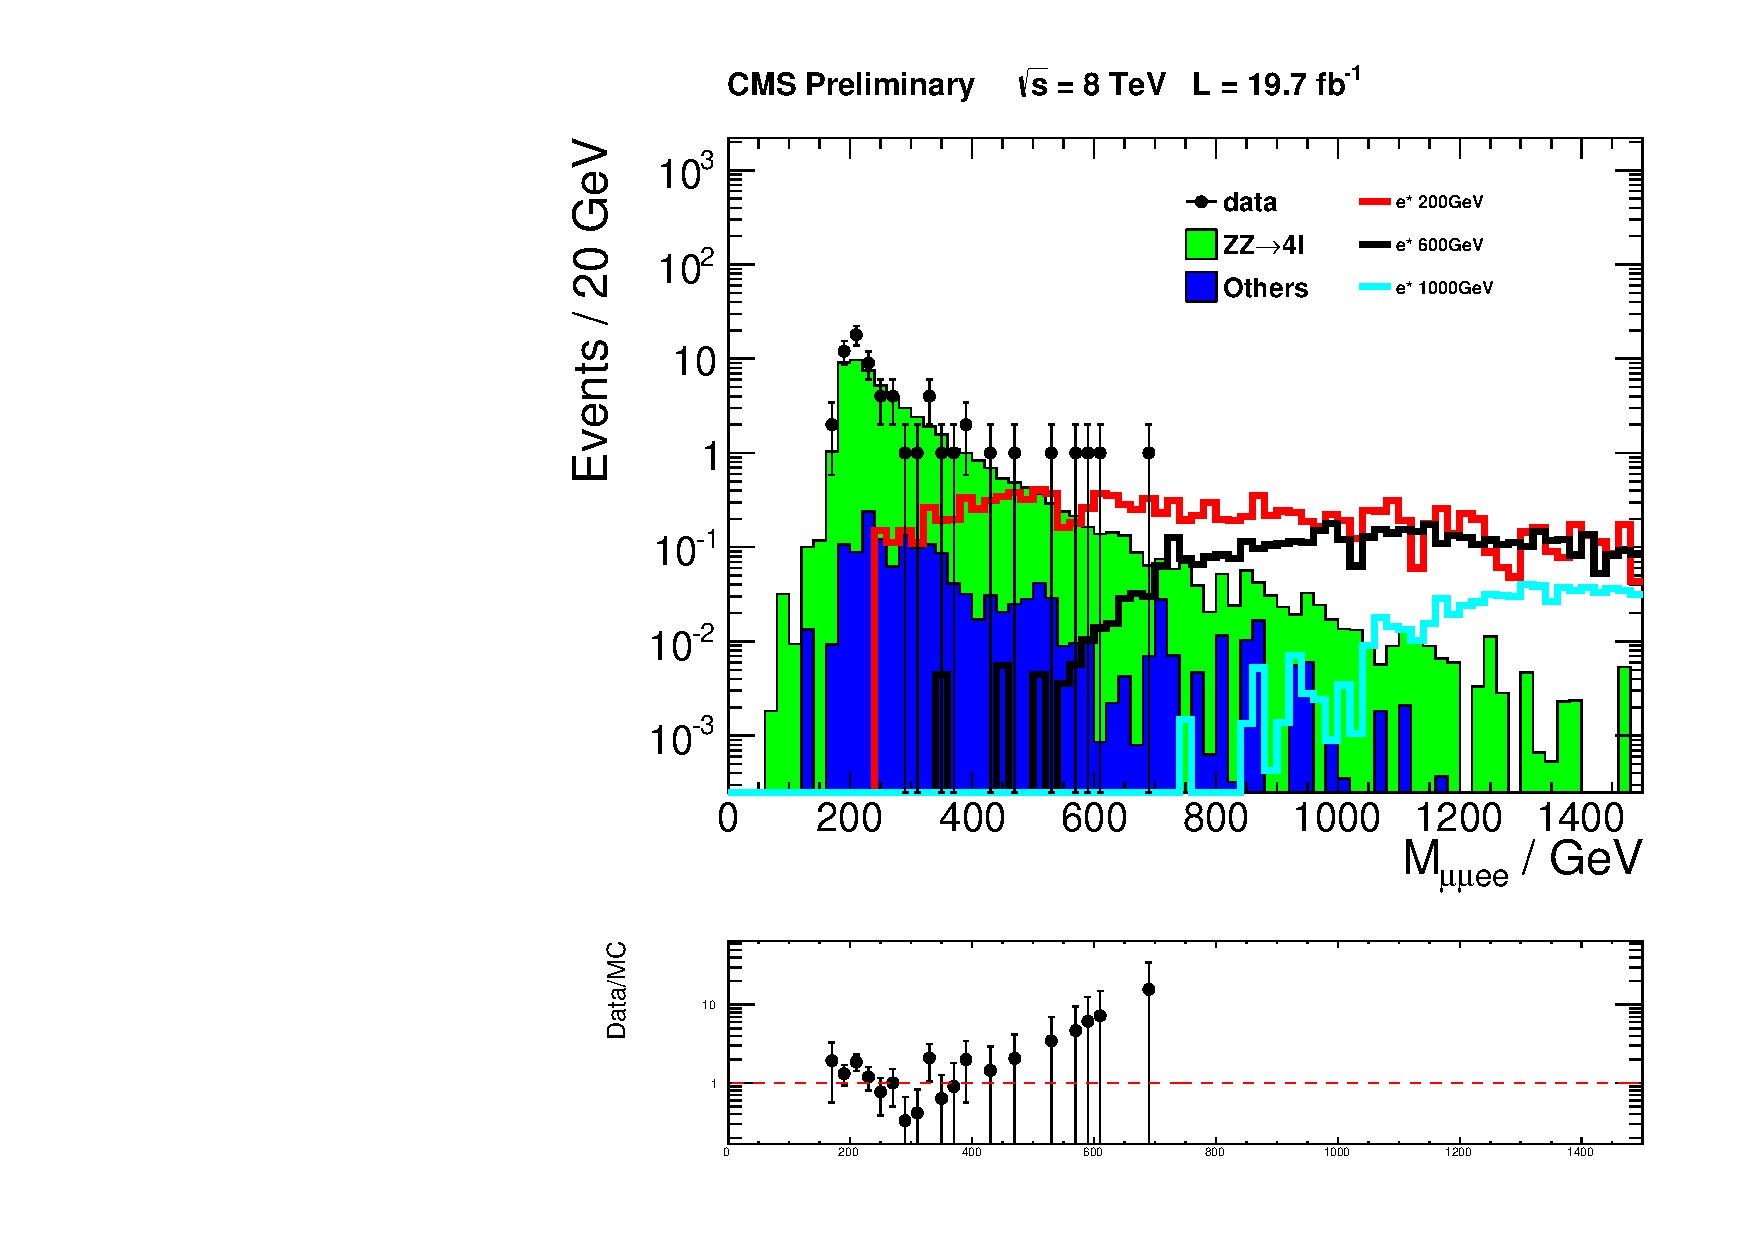
\includegraphics[width=0.48\textwidth]{plot/Minv_2mu2e.pdf} 
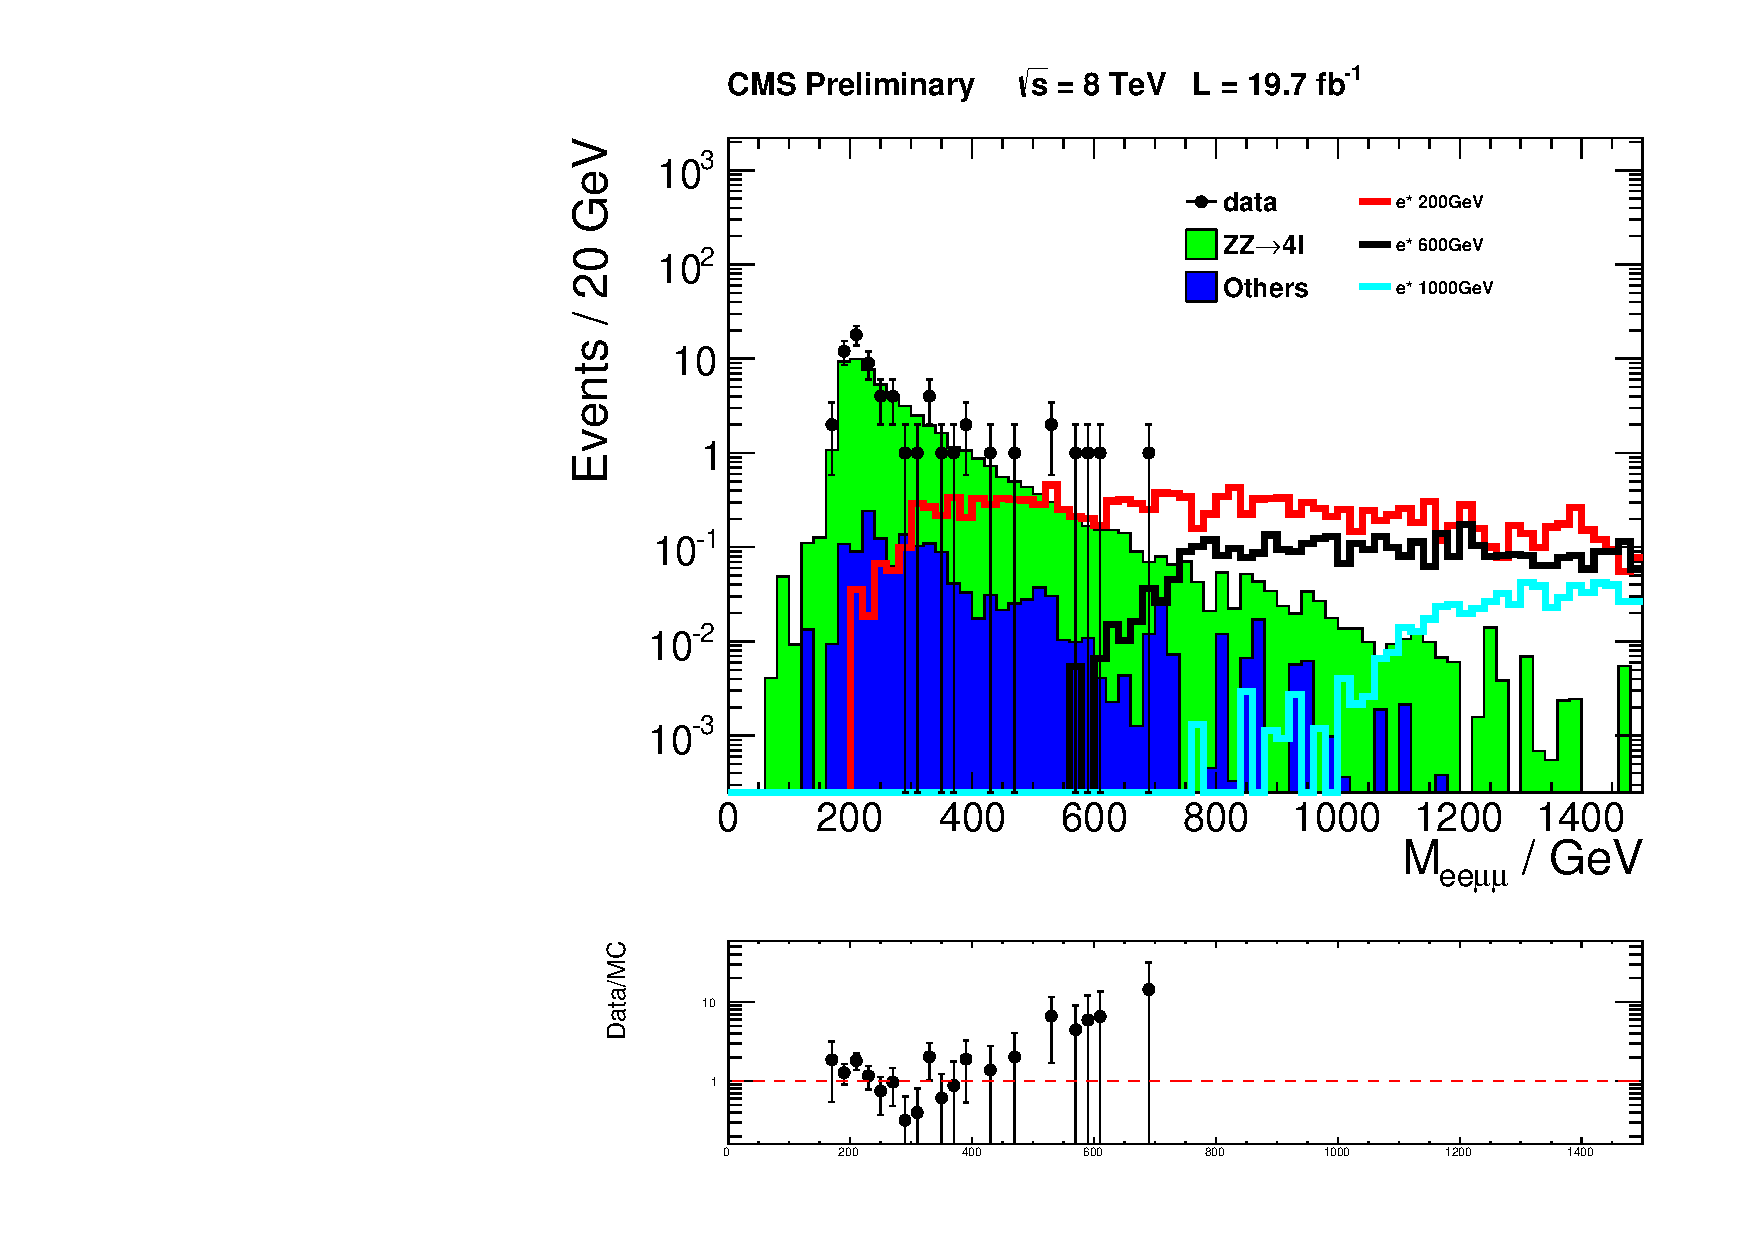
\includegraphics[width=0.48\textwidth]{plot/Minv_2e2mu.pdf}
\end{center}
\caption{\label{fig:Minv4mu}Four lepton invariant mass $M_{4l}$ before invariant mass cuts. Left: $\mu\mu^{*}\rightarrow 2\mu2e$ channel, Right: $ee^{*}\rightarrow 2e2\mu$ channel}
\end{figure}


\begin{figure}[hp!]
\begin{center}
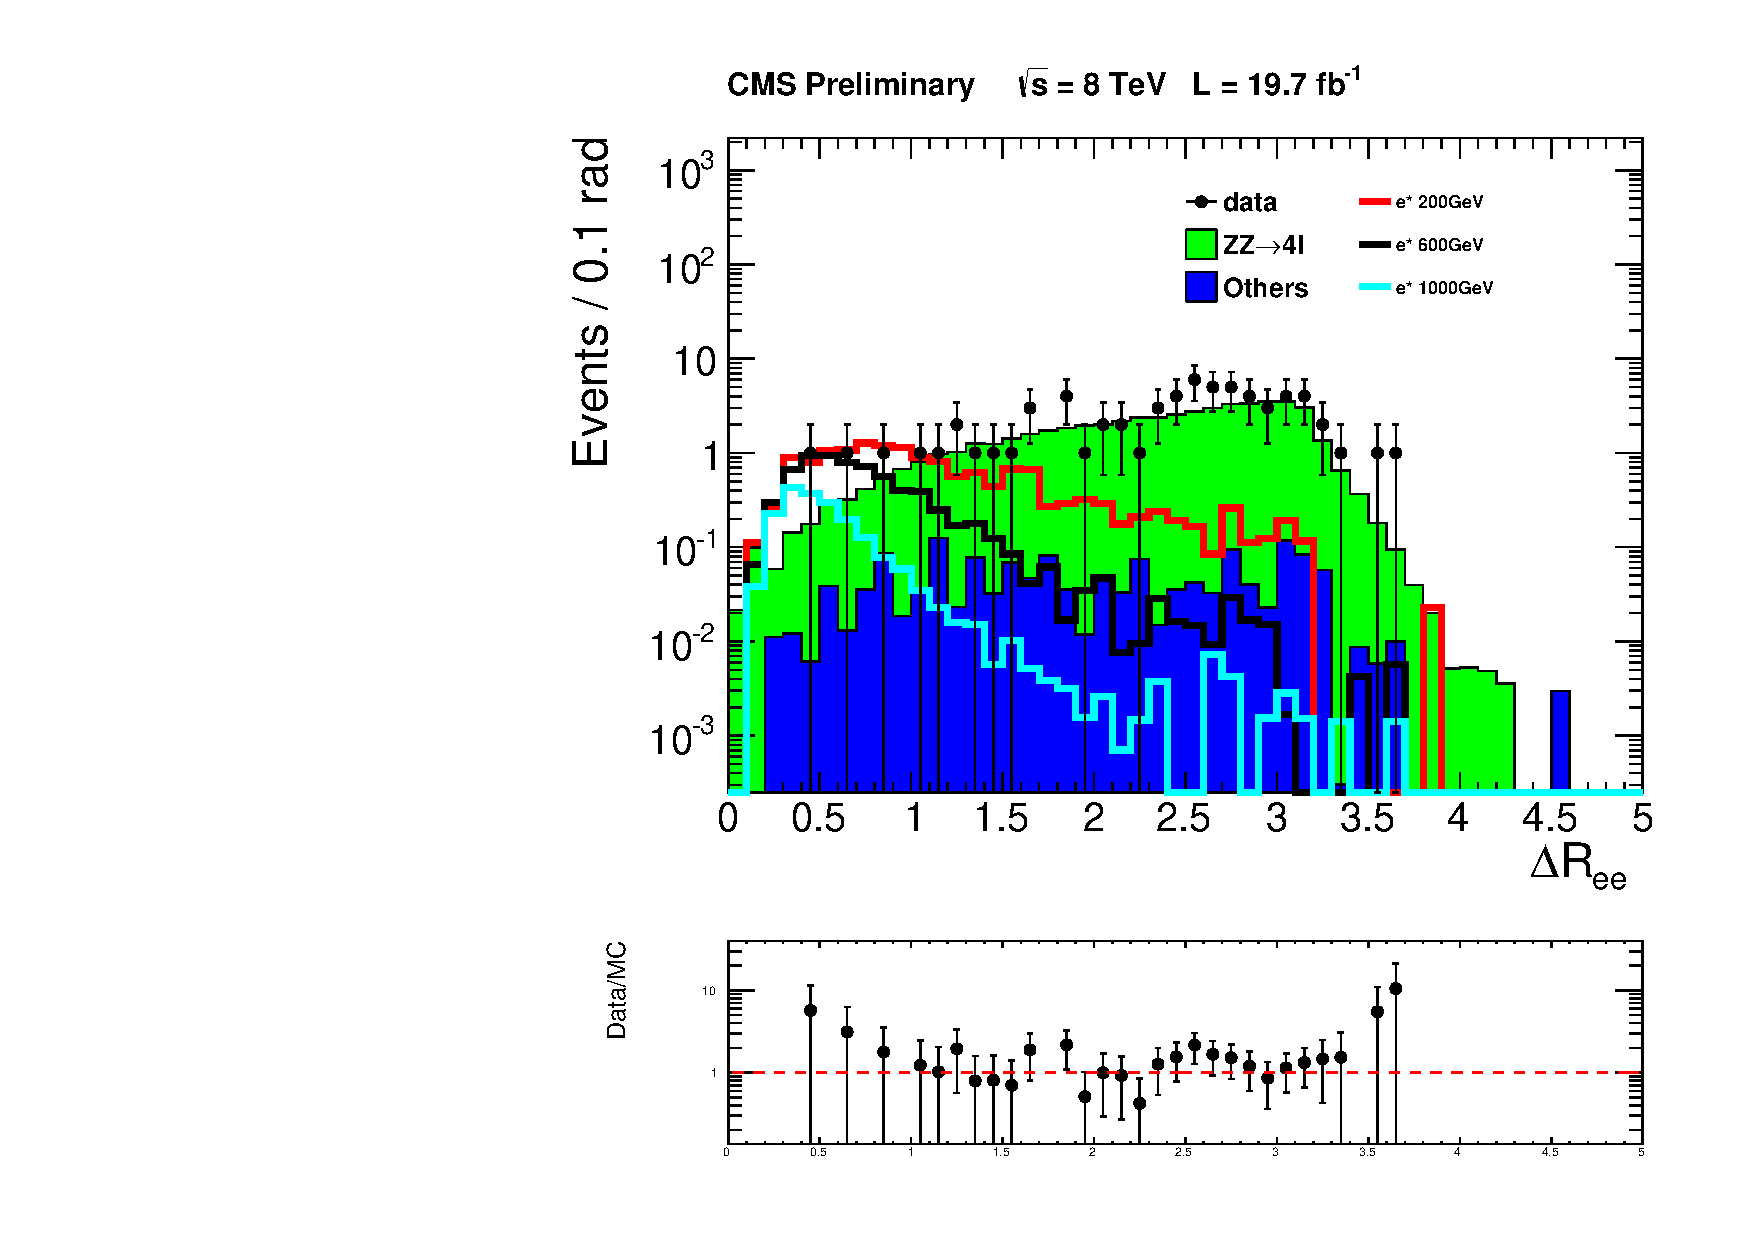
\includegraphics[width=0.48\textwidth]{plot/dR_Z_2mu2e.pdf} 
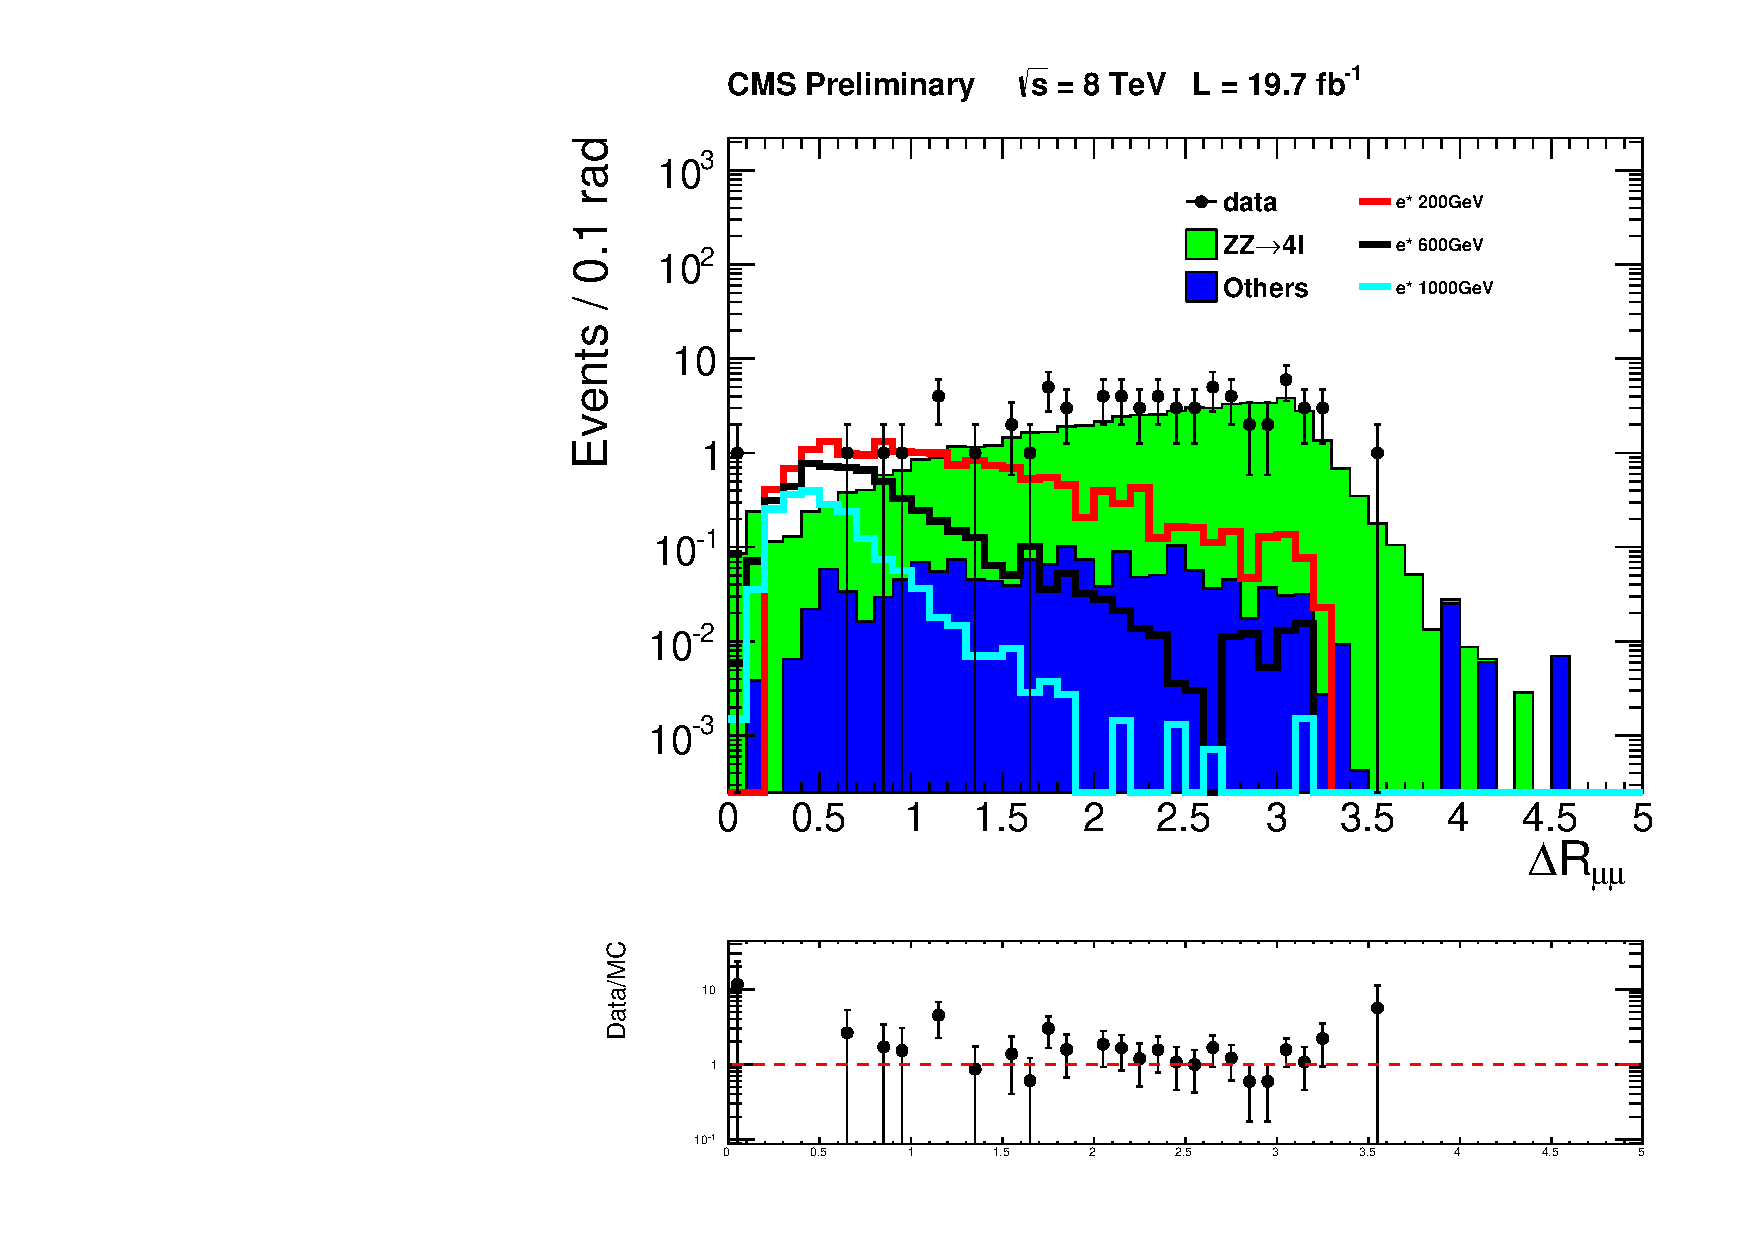
\includegraphics[width=0.48\textwidth]{plot/dR_Z_2e2mu.pdf}
\end{center}
\caption{\label{fig:ZdR}$\Delta R$ of the two muons from the Z decay before invariant mass cuts. Left: $\mu\mu^{*}\rightarrow 2\mu2e$ channel, Right: $ee^{*}\rightarrow 2e2\mu$ channel}
\end{figure}

\begin{figure}[h!]
\begin{center}
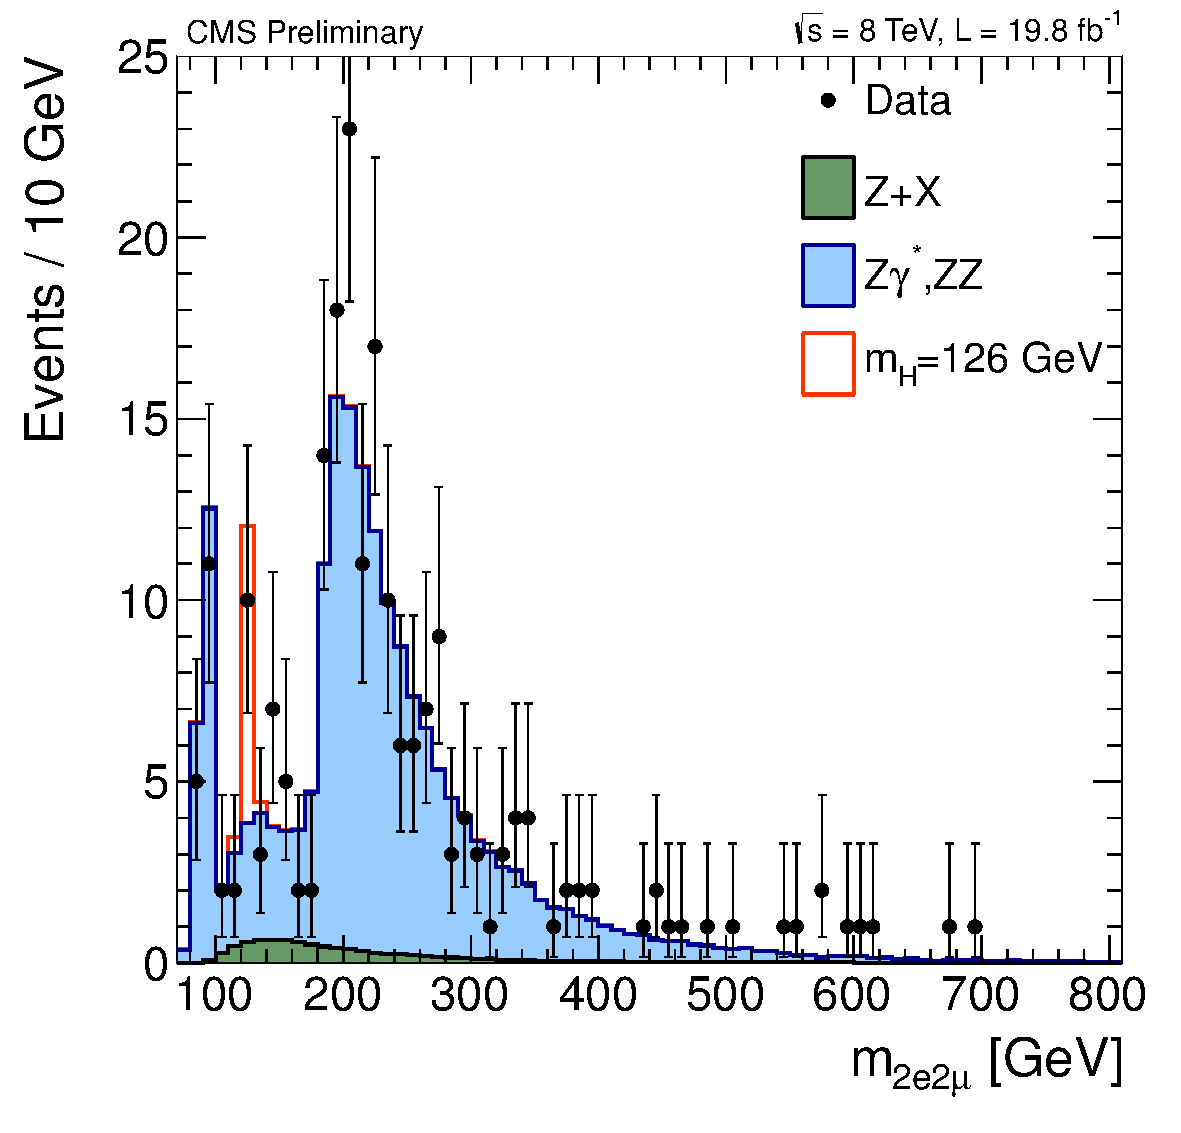
\includegraphics[width=0.6\textwidth]{plot/2e2muZZMass_70-800_8TeV.pdf}
\end{center}
\caption{\label{fig:HIGref}Four lepton invariant mass distribution in $H\rightarrow$$ZZ$$\rightarrow 2e2\mu$. The excess can also be observed around peak region.}
\end{figure}

\clearpage

\subsection*{After invariant mass cuts}

Before applying the final selection, event yields after applying the two invariant mass cuts below is concerned.

\begin{itemize}
	\item Mass cut on Z selection: $M_{Z} >$ 60 GeV
	\item Z-Veto on non-Z pair: $M_{nonZ} >$ 106 GeV
\end{itemize}

In Fig. \ref{fig:Mmin} and Fig. \ref{fig:Mmax} the minimum and maximum mass distribution are shown. One can also see the excited lepton mass from these plots by the shape of signal samples. Tab. \ref{tab:yieldsmustarZ} shows the event yields for the $\mu^{}$ channels and Tab. \ref{tab:yieldsestarZ} shows the event yields for the $e^{*}$ channels. As one can see, there are is only a small number of events left. The agreement between data and MC is good at this point of the analysis for all channels. 

\begin{table}[h!]
\begin{center}
\begin{tabular}{|l|l|l|l|}
\hline 
Background & $\mu\mu^{*}\rightarrow 4\mu$ & $\mu\mu^{*}\rightarrow 2\mu 2e$ & combined \\ 
\hline
$ZZ \rightarrow 4\mu$ & $3.45\pm 0.06$ & $0.00\pm 0.00$ & $3.45\pm 0.06$ \\
$ZZ \rightarrow 2e 2\mu$ & $0.00\pm 0.00$ & $2.14\pm 0.07$ & $2.14\pm 0.07$\\
$ZZ \rightarrow 2\mu 2\tau$ & $0.02\pm 0.01$ & $0.00\pm 0.00$ & $0.02\pm 0.01$\\
$WZ \rightarrow 3l \nu$ & $0.00\pm 0.00$ & $0.02\pm 0.01$ & $0.02\pm 0.01$\\
$gg \rightarrow ZZ \rightarrow 2l2l'$ & $0.00\pm 0.00$ & $0.11\pm 0.01$ & $0.11\pm 0.01$\\
$gg \rightarrow ZZ \rightarrow 4l$ & $0.13\pm 0.01$ & $0.00\pm 0.00$ & $0.13\pm 0.01$\\
$ttZ$ & $0.31\pm 0.08$ & $0.16\pm 0.05$ & $0.47\pm 0.09$\\
$WWZ$ & $0.08\pm 0.02$ & $0.09\pm 0.02$ & $0.17\pm 0.03$\\
$WZZ$ & $0.01\pm 0.00$ & $0.01\pm 0.00$ & $0.02\pm 0.00$\\
%$ZZZ$ & $0.00\pm 0.00$ & $0.00\pm 0.00$ & $0.00\pm 0.00$\\
\hline
Total & $4.00\pm 0.11$ & $2.53\pm 0.09$ & $6.53\pm 0.14$\\
Total (with systematics) & $4.00\pm 0.52$ & $2.53\pm 0.34$ & $6.53\pm 0.62$\\
\hline
\hline
Data & 4 & 2 & 6\\
\hline
\hline
$M_{\mu^{*}}$ = 200 GeV & $2.8 \times 10^{5}$ & $2.0 \times 10^{5}$ & $4.8 \times 10^{5}$\\
$M_{\mu^{*}}$ = 1000 GeV & $1.1 \times 10^{2}$ & $9.0 \times 10^{1}$ & $2.0 \times 10^{2}$\\
$M_{\mu^{*}}$ = 1800 GeV & 1.34 & 1.05 & 2.39\\
$M_{\mu^{*}}$ = 2600 GeV & 0.04 & 0.03 & 0.07\\
\hline
\end{tabular}
\end{center}
\caption{\label{tab:yieldsmustarZ}Events yields for $\mu\mu^{*}\rightarrow 4\mu$ and $\mu\mu^{*}\rightarrow 2\mu 2e$ after invariant mass cuts. If the column includes $0.00 \pm 0.00$ events, the calculated number is to small for a prediction.}
\end{table}


\begin{table}[h!]
\begin{center}
\begin{tabular}{|l|l|l|l|}
\hline 
Background & $e e^{*}\rightarrow 4e$ & $e e^{*}\rightarrow 2e 2\mu$ & combined \\ 
\hline
$ZZ \rightarrow 4e$ & $2.66\pm 0.05$ & $0.00\pm 0.00$ & $2.66\pm 0.05$\\
$ZZ \rightarrow 2e 2\mu$ & $0.00\pm 0.00$ & $2.32\pm 0.07$ & $2.32\pm 0.07$\\
$ZZ \rightarrow 2e 2\tau$ & $0.02\pm 0.01$ & $0.00\pm 0.00$ & $0.02\pm 0.01$\\
$ZZ \rightarrow 2\mu 2\tau$ & $0.00\pm 0.00$ & $0.02\pm 0.01$ & $0.02\pm 0.01$\\
$WZ \rightarrow 3l \nu$ & $0.03\pm 0.02$ & $0.21\pm 0.05$ & $0.24\pm 0.05$\\
$gg \rightarrow ZZ \rightarrow 2l2l'$ & $0.00\pm 0.00$ & $0.14\pm 0.01$ & $0.14\pm 0.01$\\
$gg \rightarrow ZZ \rightarrow 4l$ & $0.12\pm 0.00$ & $0.00\pm 0.00$ & $0.12\pm 0.00$\\
$ttZ$ & $0.13\pm 0.05$ & $0.12\pm 0.05$ & $0.25\pm 0.08$\\
$WWZ$ & $0.00\pm 0.00$ & $0.10\pm 0.02$ & $0.10\pm 0.02$\\
$WZZ$ & $0.01\pm 0.01$ & $0.01\pm 0.00$ & $0.02\pm 0.01$\\
%$ZZZ$ & $0.00\pm 0.00$ & $0.00\pm 0.00$ & $0.00\pm 0.00$\\
\hline
Total & $2.95\pm 0.07$ & $2.94\pm  0.10$ & $5.89\pm 0.12$ \\
Total (with systematics) & $2.95\pm 0.41$ & $2.94\pm 0.39$ & $5.89\pm 0.57$\\
\hline
\hline
Data & 0 & 4 & 4\\
\hline
\hline
$M_{e^{*}}$ = 200 GeV & $2.0 \times 10^{5}$  & $2.1 \times 10^{5}$ & $4.1 \times 10^{5}$\\
$M_{e^{*}}$ = 1000 GeV & $7.6 \times 10^{1}$ & $8.6 \times 10^{1}$ & $1.6 \times 10^{2}$\\
$M_{e^{*}}$ = 1800 GeV & 0.84 & 1.06 & 1.90\\
$M_{e^{*}}$ = 2600 GeV & 0.03 & 0.03 & 0.06\\
\hline
\end{tabular}
\end{center}
\caption{\label{tab:yieldsestarZ}Events yields for $e e^{*}\rightarrow 4e$ and $e e^{*}\rightarrow 2e 2\mu$ after invariant mass cuts. If the column includes $0.00 \pm 0.00$ events, the calculated number is to small for a prediction.}
\end{table}

\begin{figure}[hp!]
\begin{center}
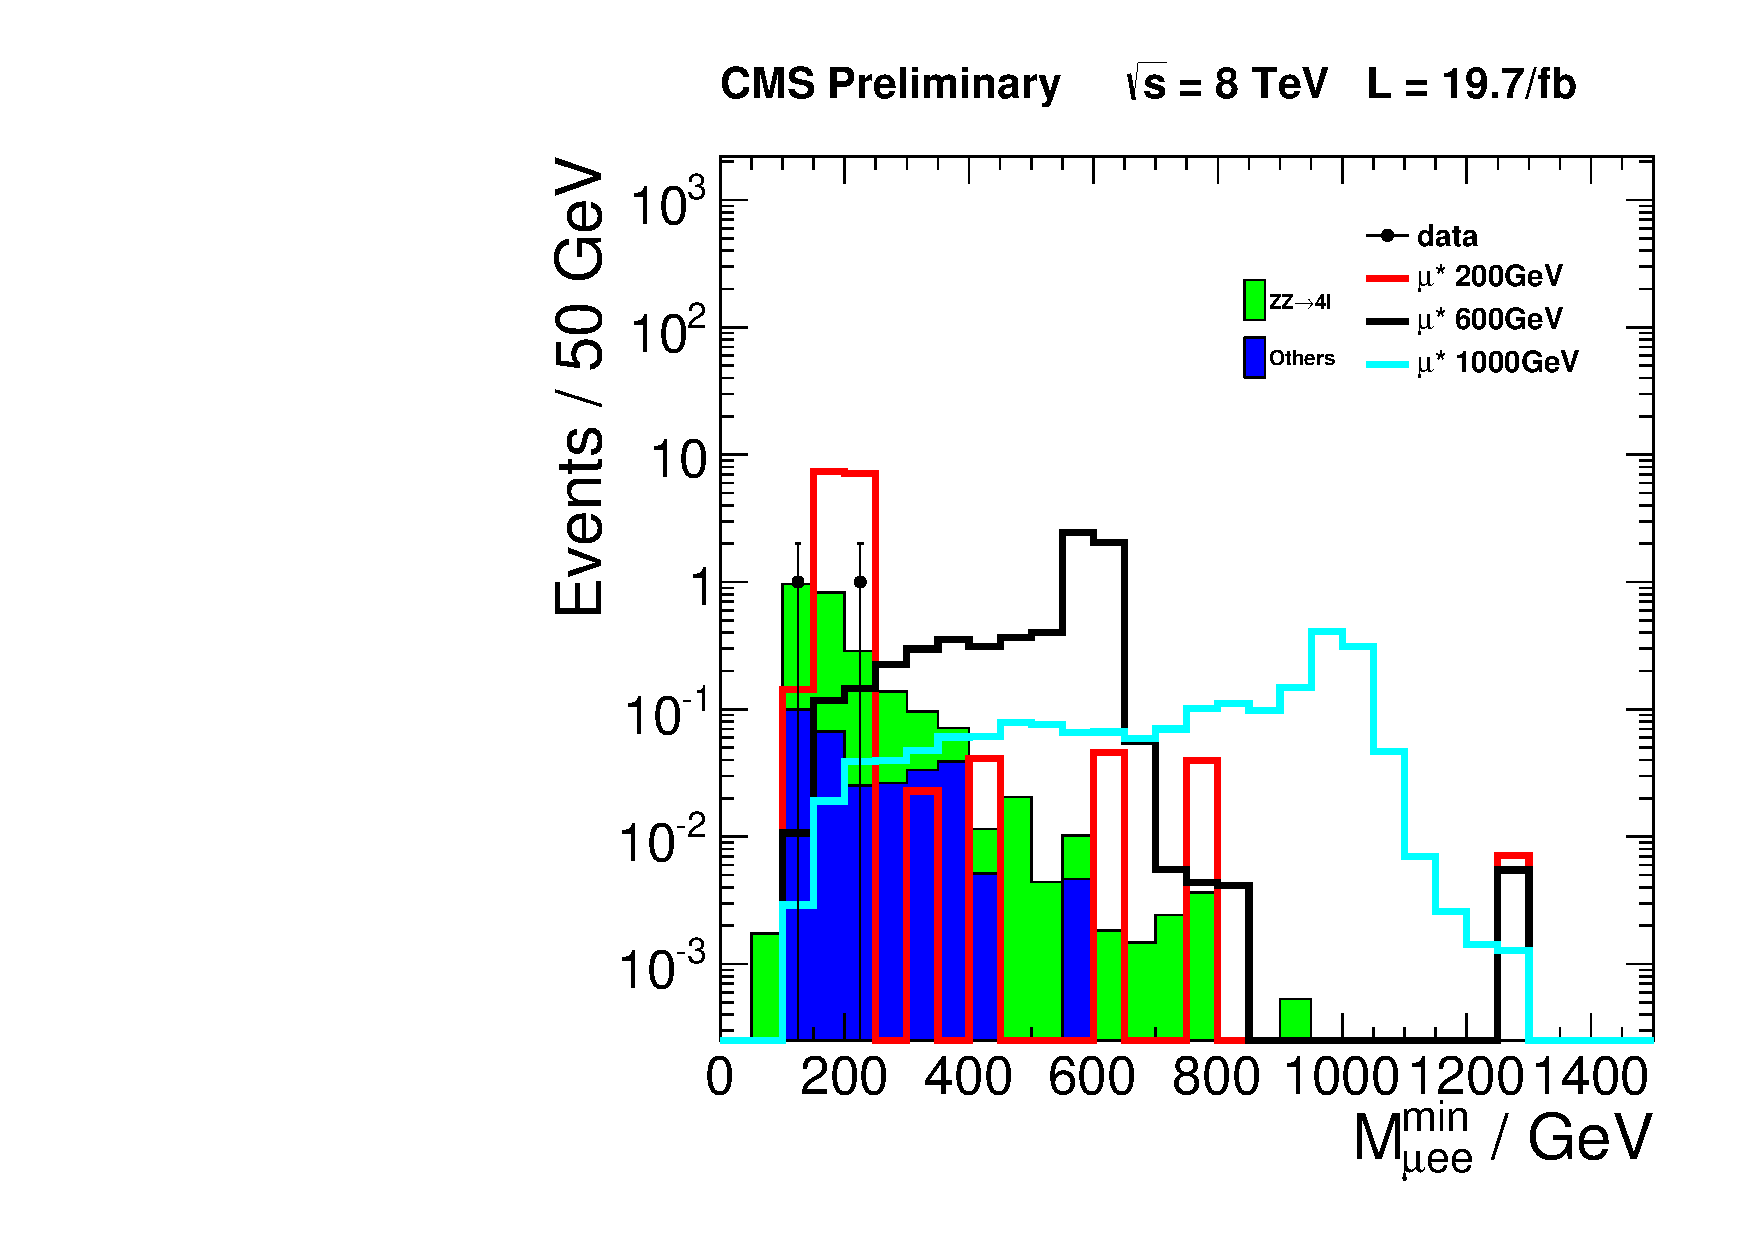
\includegraphics[width=0.48\textwidth]{plot/Mmin_2mu2e.pdf} 
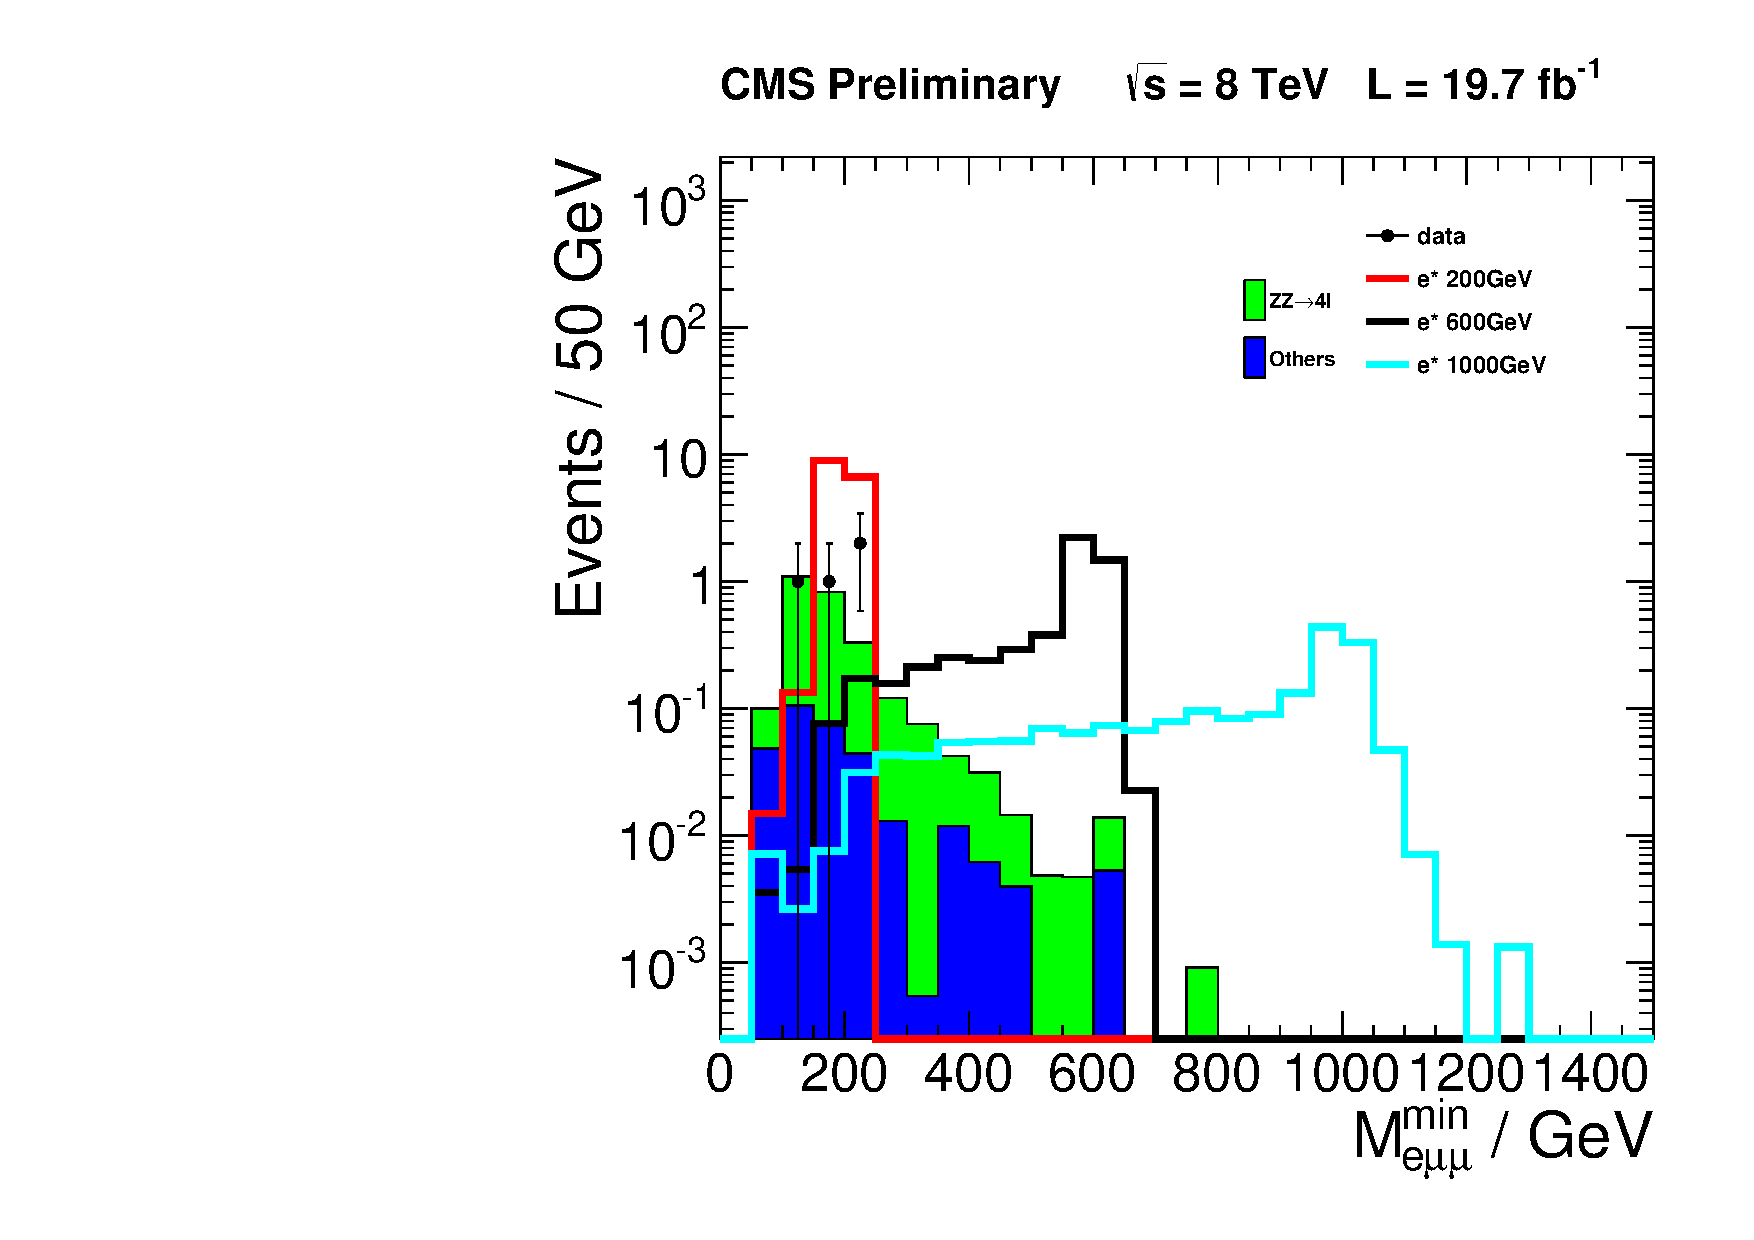
\includegraphics[width=0.48\textwidth]{plot/Mmin_2e2mu.pdf}
\end{center}
\caption{\label{fig:Mmin}Minimum invariant mass distribution $M_{min}^{3l}$ after invariant mass cuts. Left: $\mu\mu^{*}\rightarrow 2\mu2e$ channel, Right: $ee^{*}\rightarrow 2e2\mu$ channel}
\end{figure}


\begin{figure}[hp!]
\begin{center}
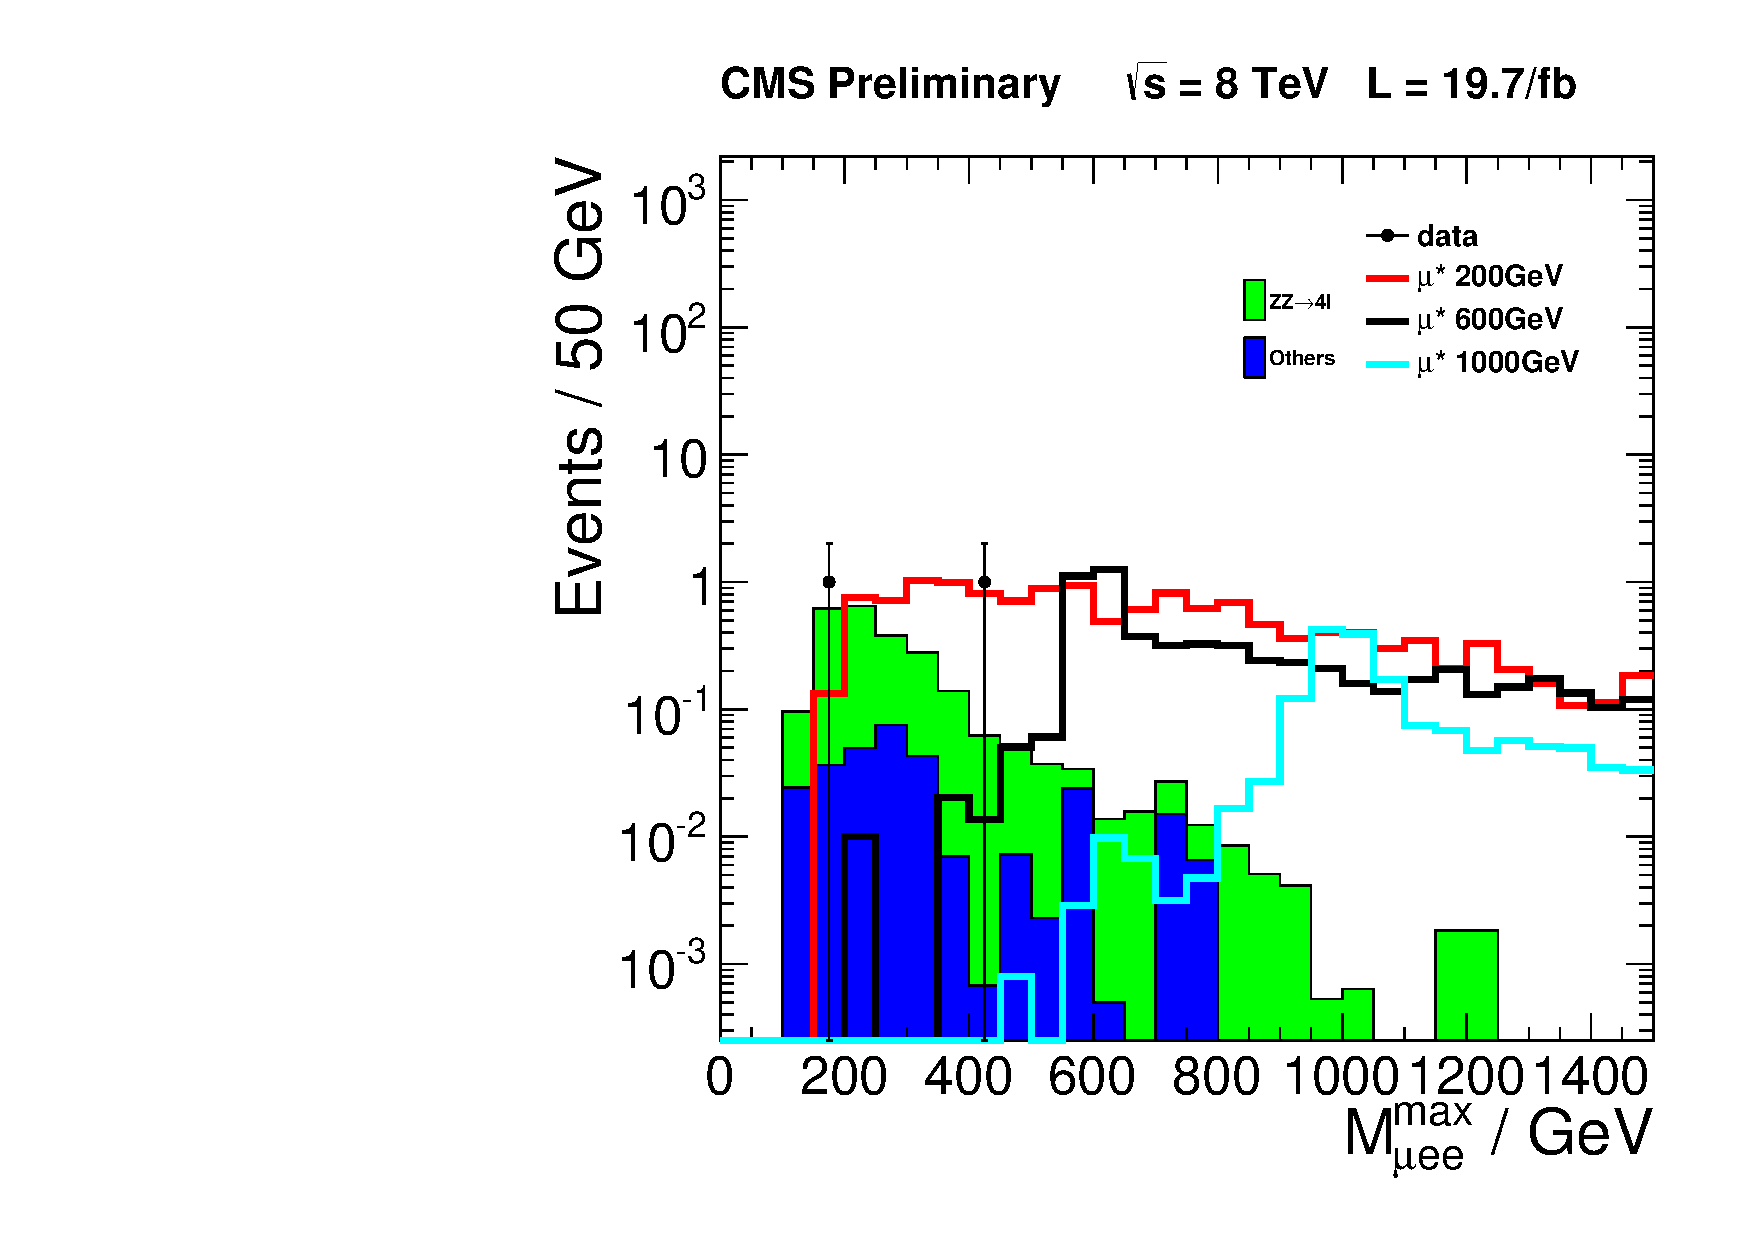
\includegraphics[width=0.48\textwidth]{plot/Mmax_2mu2e.pdf} 
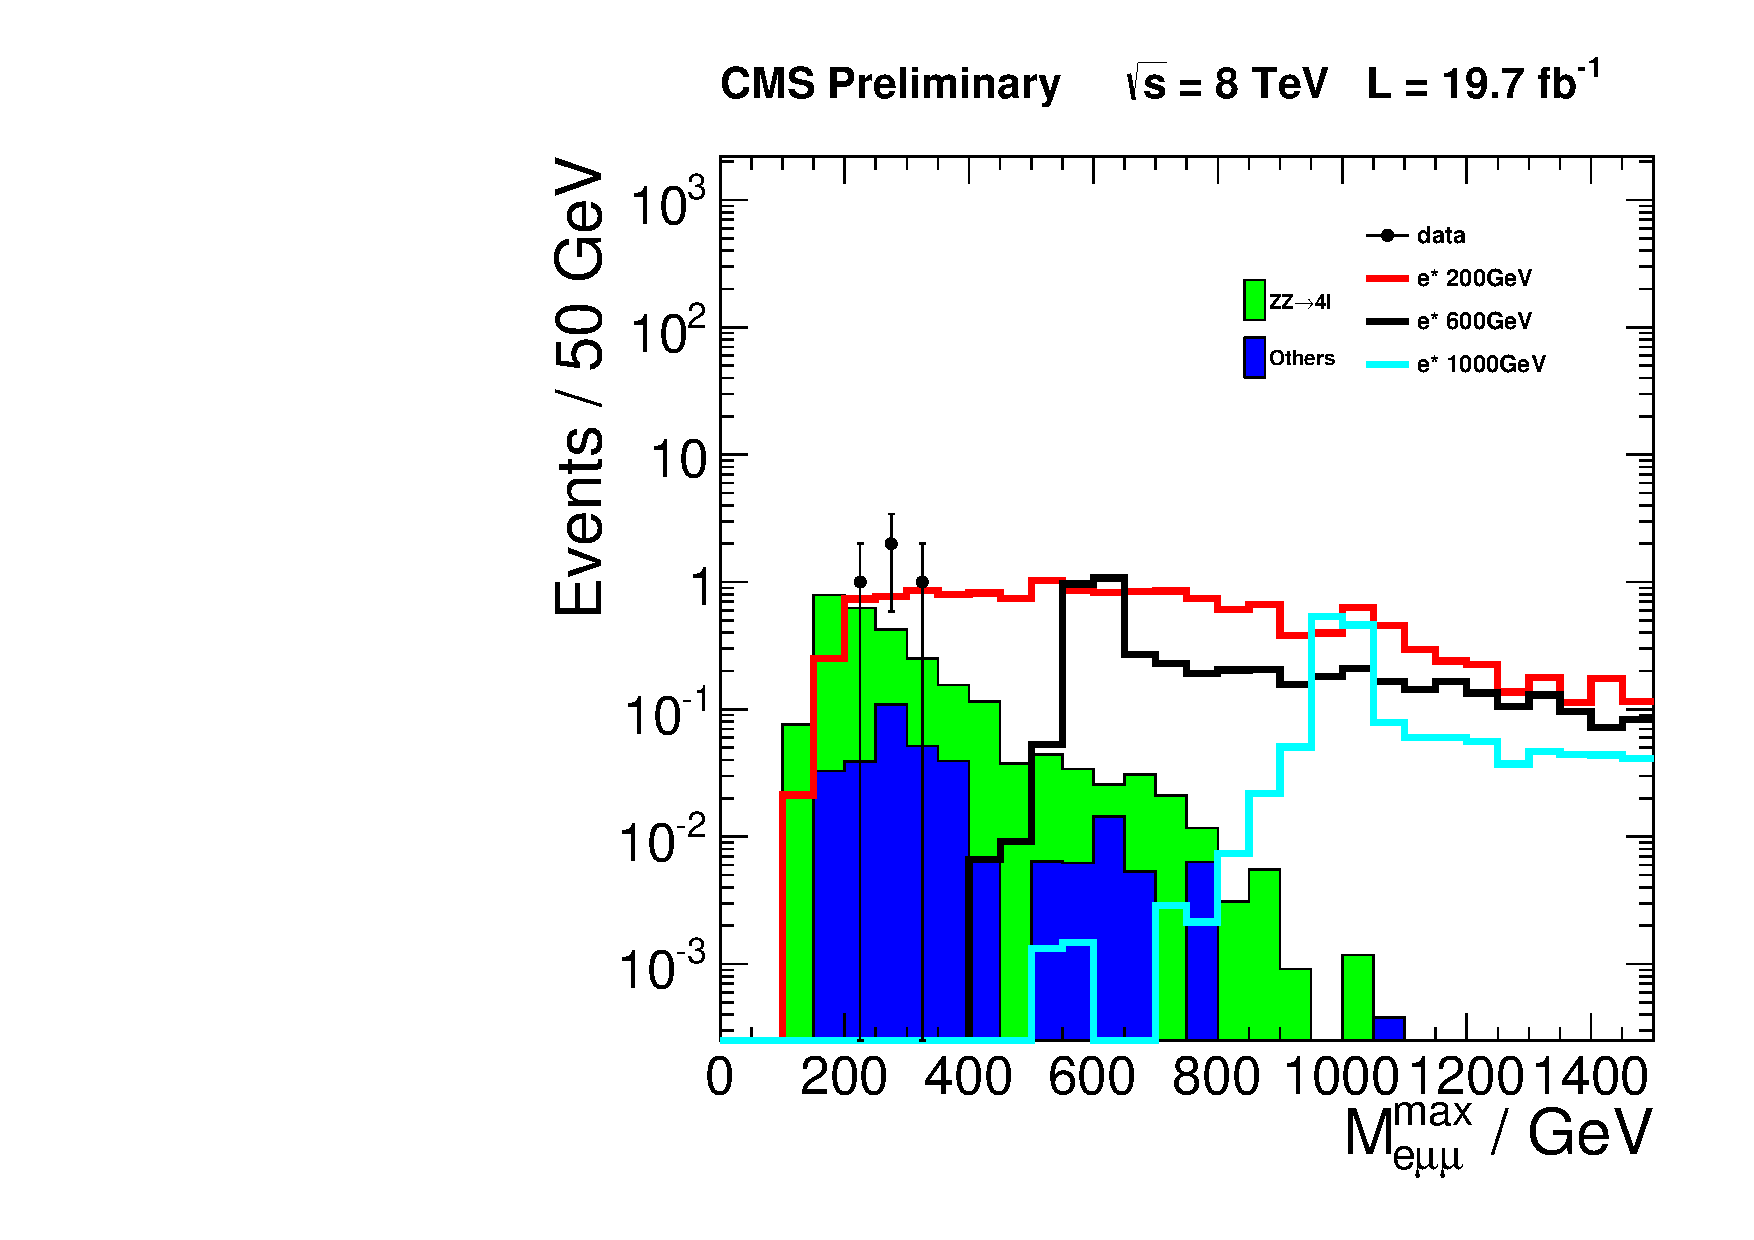
\includegraphics[width=0.48\textwidth]{plot/Mmax_2e2mu.pdf}
\end{center}
\caption{\label{fig:Mmax}Maximum invariant mass distribution $M_{max}^{3l}$ after invariant mass cuts. Left: $\mu\mu^{*}\rightarrow 2\mu2e$ channel, Right: $ee^{*}\rightarrow 2e2\mu$ channel}
\end{figure}

\newpage
